% Article template for Mathematics Magazine
\documentclass[oneside,reqno]{amsart}

%for the git double slash
\usepackage{stmaryrd}
\usepackage[colorlinks]{hyperref}
\usepackage{amsmath}
\usepackage{amssymb}
\usepackage{amsthm}
\usepackage{mathtools}
\usepackage{relsize}
\usepackage{tikz-cd}
\usepackage{graphicx}
\usepackage{caption}
\usepackage{subcaption}
\usepackage{comment}
\usepackage{nicematrix}



% These colours are tried and tested for titles and headers. Don't
% over use color!
\usepackage{color}
\definecolor{DarkBlue}{rgb}{0.1,0.1,0.5}
\definecolor{Red}{rgb}{0.9,0.0,0.1}
\definecolor{headingcol}{rgb}{0.5,0.7,1}
%\definecolor{boxcol}{rgb}{0.3,0.8,0.1}

\newtheorem{thm}{Theorem}[section]
\newtheorem{theoremdefinition}{Theorem / Definition}[section]
\newtheorem{prop}{Proposition} [section]
\newtheorem{corollary}{Corollary} [section]
\newtheorem{lemma}{Lemma} [section]
\theoremstyle{definition}
\newtheorem{definition}{Definition}[section]
\theoremstyle{definition}
\newtheorem{conjecture}{Conjecture}[section]
\theoremstyle{definition}
\newtheorem{example}{Example} [section]
\theoremstyle{definition}
\newtheorem{remark}{Remark} [section]


\newcommand{\defeq}{\mathrel{\mathop:}=}
\newcommand{\CC}{\mathbb{C}}
\newcommand{\Spec}{\text{Spec}}
\newcommand{\Proj}{\text{Proj}}
\newcommand{\PP}{\mathbb{P}}
\newcommand{\A}{\mathbb{A}}
\newcommand{\Z}{\mathbb{Z}}
\newcommand{\Os}{\mathcal{O}}
\newcommand{\Ls}{\mathcal{L}}
\newcommand{\Es}{\mathcal{E}}
\newcommand{\Fs}{\mathcal{F}}
\newcommand{\R}{\mathbb{R}}
\renewcommand{\baselinestretch}{1.2}
%This is the command that spaces the manuscript for easy reading
\title{Brane Monodromy for Toric GIT}
\author[]{Michela Barbieri}
\pagestyle{plain}
\begin{document}
\maketitle
\tableofcontents

\begin{abstract}
    Given a toric Calabi-Yau GIT problem, we have a construction for the parameter space over which mirror Landau Ginzburg models live, called the Fayet-Iliopoulos Parameter Space ($FIPS$). It is conjectured that the fundamental groupoid of $FIPS$ acts on the derived categories of the GIT quotients via spherical twists about spherical functors and line bundle twists. This is an expository report on this conjecture, where we compute a rank 2 example in detail.
\end{abstract}

\paragraph*{Acknowledgment}
I would like to give a special thanks to my PhD supervisor Professor Ed Segal for his guidance and support throughout my PhD so far. Much of the content of this report was patiently taught to me by him. 

\section{Introduction}
When mathematicians talk about mirror symmetry, they refer to a collection of mysterious relationships between different geometric objects spanning differential, symplectic, and algebraic geometry. The story starts in 1991 when string theorists Candelas, de la Ossa, Green, and Parkes published their famous paper \cite{mirrorsym}. This paper caught the attention of mathematicians because the physicists used mysterious methods to carry out calulations that they had been unable to do. \\
\newline
The question was, what was the number $n_d$ of degree $d$ curves on the quintic threefold $X \defeq \{{x_0}^5 + {x_1}^5 + {x_2}^5 + {x_3}^5 + {x_4}^5 = 0\} \subset \PP^4$? Mathematicians had only been able to work out $n_d$ for $d <4 $ and were unsure whether the number was even finite for higher $d$. In \cite{mirrorsym}, physicists computed $n_d$ for $d < 11$, with the first three numbers matching those the mathematicians had worked out. The physicists' techniques seemed like magic to the mathematicians, and the study of their work since then has resulted in a plethora of new and interesting mathematics. \\
\newline 
The rough physics is as follows. Given a Calabi-Yau manifold $(X,J,\omega)$\footnote{The $J:TX \to TX$ here is an almost complex structure on the manifold $X$. This introduces a multiplication by $i$ to tangent spaces of $X$ $(J^2 = -Id)$. $\omega$ is a symplectic form, which is a non-degenerate 2-form. We require $\omega$ to be compatible with $J$ (in which case we call $\omega$ a Kähler form) and the Calabi-Yau condition means that \textit{canonical bundle} of $X$ is trivial.} (we sometimes just write $X$ for short), string theory constructs a $\mathcal{N}=(2,2)$ \textit{super conformal field theory} (SCFT). This construction was first introduced in \cite[Section 6]{scft} in 1960. It is called a string theory because point particles in $X$ are replaced with 1-real-dimensional strings in $X$. As the strings propagate, they trace out 2-dimensional surfaces. $\mathcal{N}=(2,2)$ is short-hand for the supersymmetry algebra which acts on our SCFT. Applying an automorphism to the supersymmetry algebra somehow constructs a ‘different' but ‘isomorphic' $\mathcal{N}=(2,2)$ SCFT. We call two SCFTs related in this way \textit{mirror symmetric}.
\begin{conjecture}[Physics mirror symmetry]
Given a Calabi-Yau threefold $(X, J, \omega)$ there exists
another Calabi-Yau threefold $(X^{v}, J^{v}, \omega^{v})$ whose corresponding $\mathcal{N}=(2,2)$ SCFT is mirror symmetric to that of $(X, J, \omega)$. We call $(X^{v}, J^{v}, \omega^{v})$ mirror to $(X, J, \omega)$.
\end{conjecture}
\noindent
This is not a precise mathematical conjecture as the mathematical language to define and relate QFTs is not rigorous: for example, it is not clear what \textit{isomorphic} SCFT really means mathematically. We are also far from knowing how to construct mirrors in general, however there are some constructions such as the SYZ mirror conjecture \cite{syz}. In simple cases, such as for toric varieties, there are proven recipes for the mirror constructions called \textit{Hori-Vafa} mirrors \cite{horivafa}. This will be the context of this report and we will discuss toric mirror symmetry in more detail later on. \\
\newline
Though imprecise as stated, the physics mirror symmetry conjecture  implies some actual mathematical relationships between $(X, J, \omega)$ and a mirror $(X^{v}, J^{v}, \omega^{v})$. The most classical one of these is a Hodge-theoretic claim about the Dolbeaut cohomology groups of the manifolds. A more modern statement that is a big area of active research right now is the homological mirror symmetry conjecture, which relates some puzzlingly different categories of $X$ and $X^v$. This was first presented by Maxim Kontsevich at the 1994 International Congress of Mathematicians. The categories are called the Fukaya category and the derived category, the former depending only on the symplectic structure and the latter depending only on the complex structure. \\
\newline
The way this relates to the physics mirror symmetry is the following. Given a SCFT coming from $(X,J,\omega)$ one can construct an associate A-model and B-model via \textit{topological twisting}, where the A-model depends only on the symplectic structure and the B-model depends only on the complex structure. If we consider open strings, then what the strings attach to are objects called ‘branes’. In the A-model, these branes are Lagrangian submanifolds (with local systems)\footnote{A half dimensional submanifold $L \subset X$ is Lagrangian if $\omega|_{L} =0$.}, while in the B-model, they are algebraic subvarieties. Via this perspective it is understood that the data of a \textit{triangulated category}\footnote{A triangulated category $\mathcal{A}$ is an additive category with a shift functor $T:\mathcal{A} \to \mathcal{A}$, and a set of \textit{distinguished triangles} $A \to B \to C \to T(A) $, $A,B,C \in \mathcal{A}$, which satisfy some conditions, see \cite[Chapter 1]{huybrechts} } is carried in both models. For the A-model this is called the Fukaya Category, denoted $\text{Fuk}(X)$, and for the B-model, this is called the derived category, denoted $D^b(X)$. Very roughly, the objects and morphisms in these categories are the following:
\begin{align*}
    \text{Ob}(\text{Fuk}(X)) =& \text{Chain complexes of Langrangian submanifolds }L \subset X. \\
    \text{Hom}_{\text{Fuk}(X)}(L,L') =& \text{A chain complex made from free linear combinations of} \\
    &\text{intersection points $L \cap L'$, with differential counting holomorphic} \\
    &\text{discs between intersection points. It is called the Floer complex} \\
    &\text{and denoted } CF(L,L'). \\
    \text{Ob}(D^b(X)) =& \text{Chain complexes of coherent sheaves on } X.\text{ These are sheaves} \\
    &\text{that are locally finitely generated modules. Examples include } \\
    &\text{vector bundles, often called locally free sheaves in this context.} \\
    \text{Hom}_{D^b(X)}(\Fs^{\bullet},\Es^{\bullet}) =& \text{Chain maps $\Fs^{\bullet} \to \Es^{\bullet}$ where we invert quasi-isomorphisms.} \\
    &\text{Quasi-isomorphisms are chain maps that induce isomorphisms} \\
    &\text{on the level of homology.}
\end{align*}
See \cite[Chapter 2]{huybrechts} for a good exposition on the bounded derived category of coherent sheaves. The mirror operation relates the A-model of $(X,J,\omega)$ to the B-model $(X^{v},J^{v},\omega^{v})$, and the B-model of $(X,J,\omega)$ to the A-model of $(X^{v},J^{v},\omega^{v})$, implying equivalences of categories
\begin{align*}
    \text{Fuk}(X) &\cong D^b(X^{v}), \\
     D^b(X) &\cong \text{Fuk}(X^{v}).
\end{align*}
Given this, if we simply start with a \textit{complex geometry}\footnote{We are deliberately being vague here but just think of an algebraic variety for now.} $X$, we can ask if there is a \text{symplectic geometry} $X^{v}$ such that 
\begin{equation}
D^b(X) \cong \text{Fuk}(X^{v})
\label{HMS}
\end{equation}
From now on, we will call an $X^v$ that satisfies \eqref{HMS} a mirror to $X$. Because we didn't specify the symplectic structure of $X$, we have a whole family of mirrors, each of which is symplectomorphic to $X^v$, but has a different complex structure. We denote the complex structure moduli space of the symplectic manifold $X^v$ by $\mathcal{M}_{\text{CS}}$. Likewise we can consider all the Kähler forms (symplectic structures) on $X$, and we call this moduli space \textit{the String Kähler Moduli Space} $\mathcal{M}_{\text{SKMS}}$\footnote{In $\mathcal{M}_{\text{SKMS}}$ of $X$ we include complexified Kahler forms and other birational models of $X$.}.\\
\newline
There is a monodromy action of $\pi_1(\mathcal{M}_{\text{SKMS}})$ on $D^b(X)$ via autoequivalence, which is the B-side `brane monodromy'. There is also a monodromy action of $\pi_1(\mathcal{M}_{\text{CS}})$ on $\text{Fuk}(X^v)$ via autoequivalence, which is the A-side `brane monodromy'. The homological mirror symmetry conjecture implies $\mathcal{M}_{\text{CS}} \cong \mathcal{M}_{\text{SKMS}}$. Since it's easier to understand $\mathcal{M}_{\text{CS}}$ rather than $\mathcal{M}_{\text{SKMS}}$, we will study how the A-side brane monodromy carries over to the B-side. \\
\newline
The way this action should carry over is not clear entirely. This is because mirror symmetry proofs don't necessarily give explicit mirror maps that we can use. The main objective of this report is to make sense of a conjecture on how this action carries over in a specific context, which is \textbf{toric Calabi Yau  Geometric Invariant Theory (GIT)}. The reason we work in this context is threefold: firstly, toric geometry is combinatorial and allows for the construction of informative yet hands-on examples; secondly, we have a heuristic recipe a parameter space called the Fayet-Iliopoulos parameter space ($FIPS$), which is closely related to $\mathcal{M}_{\text{CS}}$; and lastly, the GIT context provides us with interesting autoequivalences, which come from so called \textit{spherical functors}.\\
\newline
Toric GIT is a theory of how to take quotients when you have an algebraic torus $T \cong (\CC^*)^r$ acting on a vector space $V\cong \CC^n$. It turns out that to get something nice, you need to remove a certain zero locus from $V$ before taking the naive topological quotient. It also turns out that this process is not unique and depends on a \textit{stability condition}, which is just a choice of character $\theta: T \to \CC^*$. Different characters will tell you to remove different loci, and therefore give birational but not isomorphic quotients (in general). We denote the quotient corresponding to stability condition $\theta$ by $X_{\theta}=V \sslash_{\theta} T$. We call the locus we remove \textit{the unstable locus}. We will explain in more detail how a stability condition determines an unstable locus in Section \ref{GIT}. By some representation theory, any character $\theta: T \to \CC^*$ is of the following form
$$
\theta(\lambda_1, \dots, \lambda_r) = {\lambda_1}^{\theta_1} \dots {\lambda_r}^{\theta_r} 
$$
where $(\theta_1, \dots, \theta_r) \in \Z^r$. So the characters live in a rank $r$ lattice $L^v$, called \textit{the character lattice}. \\
\newline
The character lattice $L^v$ splits into positive cones where any two stability conditions lying in the interior of the same cone have the same unstable locus. The top dimensional cones correspond to good quotients in the sense that they are smooth Deligne-Mumford stacks (the stabilisers are finite groups). The GIT quotients corresponding to the top dimensional cones are therefore the ones we mean when we discuss the collection of GIT quotients. We call the decomposition of $L^v$ \textit{a wall and chamber decomposition}, where note two GIT quotients are said to separated by a wall if their cones share a codimension 1 face.\\
\newline
We note that the wall and chamber decomposition of $L^v$ gives us the data of a toric fan, which we call \textit{the secondary toric fan}. The geometric realisation of this fan is a toric variety $\Fs$ which we call the \textit{secondary toric variety}. By toric orbit-cone correspondence, fixed points in $\Fs$ under the dual torus $T^v$ action correspond to GIT quotients.  \\
\newline
Let us consider a wall $W$ in the secondary fan separating two GIT quotients $X$ and $X'$. The \textit{wall-crossing formula}, which we explain in more detail in Section \ref{wallcrossing}, tells us that
$$
D^b(X) = \langle D^b(X'), D^b(Z),...,D^b(Z) \rangle_{SOD}
$$
where $Z$ is the $T$-quotient of the fixed locus of the action of the one-parameter familly perpendicular to the wall, and the number of copies of $Z$ can be easily computed combinatorially\footnote{In fact, $Z$ comes from a GIT problem called a \textit{Higgs GIT problem}, whose data is a subset of the data of our original GIT problem. We will explain this in more detail in Section \ref{wallcrossing}.}. We may call $X'$ \textit{minimal} with respect to $X$, and $X$ \textit{maximal} with respect to $X'$. \\
\newline
A toric Calabi-Yau GIT problem is a toric GIT problem where the sum of the weights is 0. This condition on the action of the torus $T$ that ensures all the quotients are Calabi-Yau i.e. that they have trivial canonical bundle. This ensures that whenever you wall cross the number of copies of $D^b(Z)$ is 0, so that all your GIT quotients are derived equivalent through wall crossing. If we fix a GIT quotient $X$, wall-crossing through a wall $W$ actually gives us countably-infinite derived equivalences between $X$ and the GIT quotient on the other side of the wall. Going through one equivalence and back through another produces a non-trivial autoequivalence of $D^b(X)$. For any wall we therefore have countably-infinitely-many non-trivial autoequivalences of $D^b(X)$. \\
\newline
Though the number of copies of $D^b(Z)$ in the SOD is 0, the toric variety $Z$ is still very important. For any wall $W$ and corresponding $Z$ we get a \textit{spherical functor}
$$
F : D^b(Z) \to D^b(X).
$$
This means that the \textit{spherical twist} $T_F: D^b(X) \to  D^b(X) $ is an autoequivalence. We will explain what $F$ and $T_F$ are in Section \ref{CY}. In \cite{gitauto}, Halpern-Leistner and Shipman proved that the autoequivalences coming from wall crossing are the same as those coming from these spherical functors. \\
\newline
Other than having a good understanding of lots of non-trivial autoequivalences of derived categories of Calabi-Yau toric GIT quotients, we also have another important tool which is that we have a recipe for the mirror. Consider a rank $r$ dimension $n$ toric Calabi-Yau GIT problem $T \cong (\CC^*)^r$ acting on $V \cong \CC^n$. The data of $T$ acting on $V$ determines a Gauged Linear Sigma Model (GLSM), a particular kind of \textit{supersymmetric 2-dimensional QFT} (SQFT). The mirror is given by a \textit{Landau Ginzburg}\footnote{Given a Landau Ginzburg model, one can also build a SQFT.} model $(({\CC}^*)^{n-r}, W) $ where $W: ({\CC}^*)^{n-r} \to \CC$ is a Laurent polynomial called the \textit{superpotential}. This mirror symmetry was described by physicists Hori-Vafa \cite{horivafa} and a corresponding homological mirror symmetry statement has been proved mathematically. The Landau Ginzburg model is a mirror in the homological sense via the equivalence of categories
\begin{equation*}
    D^b(X) \cong \text{FS}(({\CC}^*)^{n-r}, W)
\end{equation*}
where $X$ is a GIT quotient and by $\text{FS}$ we mean the \textit{Fukaya-Seidel Category}, or \textit{the Fukaya category with stops} \cite{seidelfukaya}.
In fact we have a family of these mirror Landau Ginzburg models, which vary by choice of coefficients of the Laurent polynomial $W$. There's a combinatorial recipe to construct the parameter space over which the mirror Landau Ginzburg models live and we call this parameter space the Fayet-Iliopoulos parameter space ($FIPS$). It is the complement of the \textit{GKZ dicriminant locus} $\Delta$ of $W$ inside the dual torus $T^v$ \cite{gelfand1994discriminants}. This discriminant generalises the well-known discriminant of the quadratic to Laurent polynomials of any type in any number of variables, which we will explain in more detail in Section \ref{fips}. \\
\newline 
An important remark is that $FIPS$ is not the same as $\mathcal{M}_{\text{CS}}$ or $\mathcal{M}_{\text{SKMS}}$, see Remark 2.8 in \cite{edwill} for an explanation of this. That said, there should be a map from $FIPS \to \mathcal{M}_{\text{CS}}$. Since $FIPS$ is the only thing we have a heuristic recipe for, we study a monodromy action of $FIPS$ on the derived categories of the GIT quotients. It is helpful to think of $FIPS$ as living inside the secondary toric variety $\Fs$. Recall that there are points in the boundary of $\Fs$ that correspond to GIT quotients. This makes the $\Fs$ an interesting compactification of $FIPS$ because we can then see limiting regions of $FIPS$ that correspond to specific GIT quotients. We can consider the fundamental groupoid of $FIPS$ $\Pi_1(FIPS)$ with a base point for every limiting region. The conjecture is that a path from one quotient $X$ to another quotient $X'$ acts on the set of derived categories of the GIT quotients via composition of wall-crossings (or spherical functor twists) and line bundle twists. Non-homotopic paths will correspond to different equivalences. \\
\newline
In Section \ref{FIPS} we will explain more details of the theory and put into plain sight how we exactly match the paths/loops in $\Pi_1(FIPS)$ to certain equivalences between the derived categories of the GIT quotients. In Section \ref{rank2example} we prove the conjecture for a rank 2 example.  \\
\newline
Finally, in Section \ref{future} we lay out our plan to prove this conjecture for toric Calabi-Yau threefolds of Picard rank 2.

\section{Background on Toric CY GIT}
\label{background}
\subsection{General Toric Geometric Invariant Theory}
\label{GIT}
We start with the algebraic torus $T \cong (\mathbb{C}^*)^r$ acting on a vector space $V \cong \mathbb{C}^n$. We call this a rank $r$ dimension $n$ \textit{toric geometric invariant theory (GIT) problem}. We would like to construct a space that parametrises the actions orbits. \textit{Geometric Invariant Theory} (GIT) is the theory that tells us \textit{the unstable locus} to throw away before we quotient so that we get a good/geometric quotient \cite{mumford1994geometric}. GIT quotients are often denoted $X \sslash G$. By the representation theory of the algebraic torus, for a choice of coordinates on $T$ and $V$ the actions must be of the form:
$$
(\lambda_1, \dots, \lambda_r) \cdot (z_1, \dots, z_n) = ({\lambda_1}^{q_{11}}{\lambda_2}^{q_{21}}\dots {\lambda_r}^{q_{r1}} z_1, \dots, {\lambda_1}^{q_{1n}}{\lambda_2}^{q_{2n}}\dots {\lambda_r}^{q_{rn}} z_1)
$$
We get an $r \times n$ integer matrix $Q = (q_{ij})$, called the \textit{weight matrix}. The column vectors $q_i = Q(e_i)$ of $Q$ are hence called the \textit{weights}.
\begin{example}
  Consider $\mathbb{C}^*$ acting on $\mathbb{C}^2$ linearly, i.e. $\lambda \cdot (x, \, y) = (\lambda x,\, \lambda y)$.
  If we take the quotient space, we see that the orbit of the origin cannot be separated from any other orbit. So we have to remove the origin and as expected, we get  GIT quotient $$ \mathbb{C}^2 \sslash \mathbb{C}^* = \mathbb{C}^2 \backslash \{(0, \, 0)\} / \mathbb{C}^* = \mathbb{P}^1$$
  \begin{figure}[!h]
    \centering
    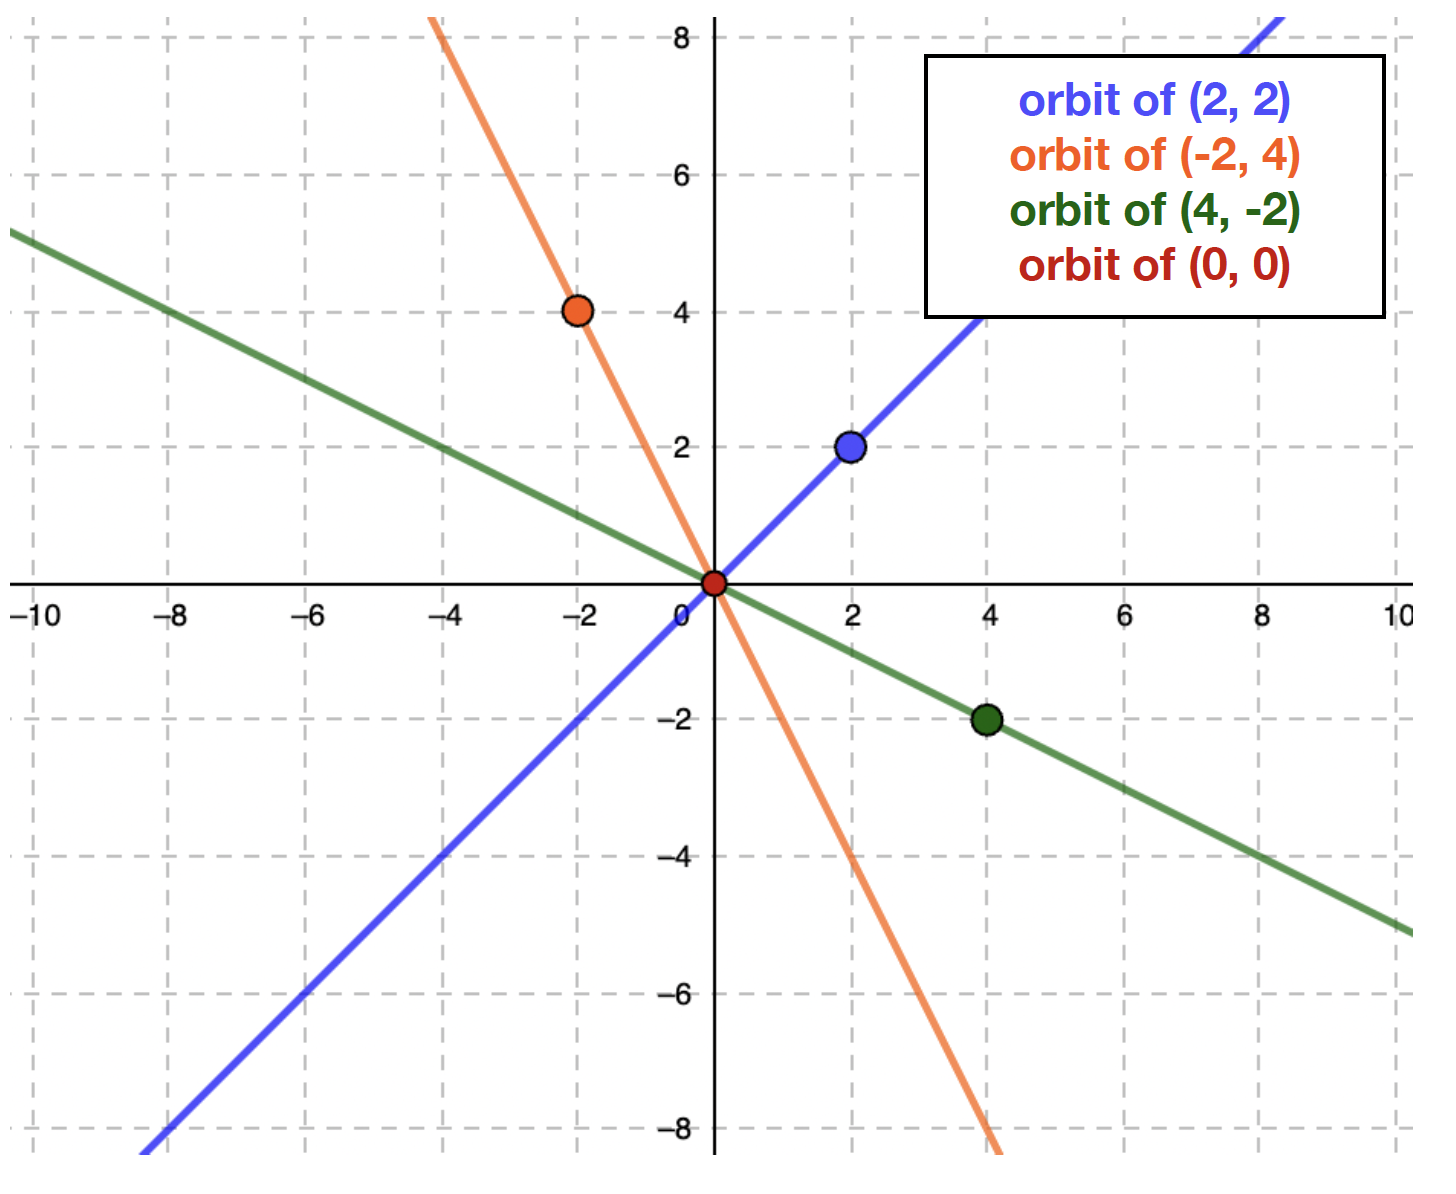
\includegraphics[width=5cm]{git/orbits of P1.png}
    \caption{Orbits of the $\mathbb{C}^*$ action on $\mathbb{C}^2$.}
  \end{figure}  
\end{example}
\noindent
In general GIT quotients are not unique and depend on a choice of \textit{stability condition}. As we explained in the introduction, in the affine GIT problem a stability condition is just a choice of character $\theta : T \to \CC^*$. Since the character lattice $\text{Hom}(T, \CC^*)$ is isomorphic to $ \Z^r$, we can see $\theta \in \mathbb{Z}^r$. Different choices of $\theta$ have us remove different unstable loci and give us non-isomorphic (but birational) quotients. This amounts to just looking at the positive cones of collections of weights $q_i$ who contain $\theta$. We will spell exactly how next, where we use Section 4 of \cite{coates2018crepant} as our main reference. \\
\newline
We will reformulate in a non-coordinate dependent way. The following is our GIT data:
\begin{itemize}
    \item $T \cong (\CC^*)^r$ a connected algebraic torus of rank $r$,
    \item $L \defeq \text{Hom}(\CC^*,T) \cong \Z^r$, the \textit{cocharacter lattice},
    \item $q_1, \dots, q_n \in L^v = \text{Hom}(T, \CC^*) \cong \Z^r $, a collection of characters we call \textit{weights}.
\end{itemize}
We call $L^v$ the \textit{character lattice}. The weights $q_1, \dots,q_n$ define a map from $T$ to $(\CC^*)^n$ and hence define an action on $\CC^n$ through the action of the torus. For a subset $I \subset \{1, 2, \dots , n\}$, and write $\bar{I}$ for the complement of $I$, and set
\begin{align}
    \angle_I =\left\{ \sum_{i\in I} a_i q_i \: \big{|} 
    \: a_i \in \mathbb{R}_{>0} \right\} \in L^v \otimes \mathbb{R}
\end{align}
where we call $\angle_I$ \textit{the strictly positive cone on weights} $\{q_i| i \in I \}$. We set $\angle_\emptyset = \{0 \}$. Consider a \textit{stability condition} $\theta \in L^v$. Set
$$
\mathcal{A}_\theta = \left\{ I \subset \{1,2,\dots,n \} \: \big{|} \: \theta \in \angle_{I}\right\}.
$$
We make the following assumptions on $\theta$:
\begin{enumerate}
    \item $\{1,2, \dots, n\} \in \mathcal{A}_\theta $,
    \item for any $I \in \mathcal{A}_\theta $, $\{q_i \: |\: i \in I \}$ spans $L^v \otimes \mathbb{R}$ over $\mathbb{R}.$
\end{enumerate}
The first ensures that our quotient won't be empty and the second ensures that we are picking a good stability condition, in that our quotient will be a smooth Deligne Mumford stack. Consider coordinates $z_1,\dots, z_n$ on $\CC^n$. We define the ideal 
$$
\mathcal{I}_{\theta} = \left\langle \prod_{i \in I} z_i  \: \big{|} \: I \in \mathcal{A}_{\theta} \right\rangle
$$
We define \textit{the unstable locus of $\theta$} to be 
$$
S_{\theta} = V(\mathcal{I}_{\theta})
$$
so that our GIT quotient is toric smooth DM stack:
$$
X_{\theta} = [ \CC^n \backslash S_\theta \: / \: T ].
$$
The space of stability conditions satisfying our assumptions has a wall and chamber structure. The chamber $C_\theta$ to which $\theta$ belongs is given by
$$
C_\theta = \bigcap_{I \in \mathcal{A}_\theta} \angle_I
$$
and $X_\theta = X_{\theta'}$ if and only if $\theta' \in C_\theta$. The GIT quotient $X_{\theta'}$ changes when we cross a codimension one boundary of $C_{\theta}$. This wall and chamber structure gives us a fan in $L^v$, which we call \textit{the secondary fan}. We note that the 1-dimensional cones may be more than just the weights of the action. Corresponding to the secondary fan is a
toric variety, the secondary toric variety $\Fs$. 
\begin{example}
  Consider $\mathbb{C}^*$ acting on $\mathbb{C}^3$ via $\lambda \cdot (x, \, y, \, z) = (\lambda x,\, \lambda y, \, \lambda^{-1}z)$. The character lattice is isomorphic to $\mathbb{Z}$. For $\theta > 0$, we have unstable locus $Z_{+} = \{ x = y = 0 \}$. We have GIT quotient $$\mathbb{C}^3 \sslash_{\theta} \mathbb{C}^* = \mathbb{C}^3 \backslash{\{ x = y = 0 \}} / \mathbb{C}^* = \mathcal{O}(-1)_{\mathbb{P}^1_{x:y}}.$$
   For $\theta < 0$, we have unstable locus $Z_{-} = \{z = 0\}$.
   $$\mathbb{C}^3 \sslash_{\theta} \mathbb{C}^* = \mathbb{C}^3 \backslash{\{ z = 0 \}} / \mathbb{C}^* = \mathbb{A}^2_{x, \, y}.$$
   \begin{figure} [!h]
    \centering
    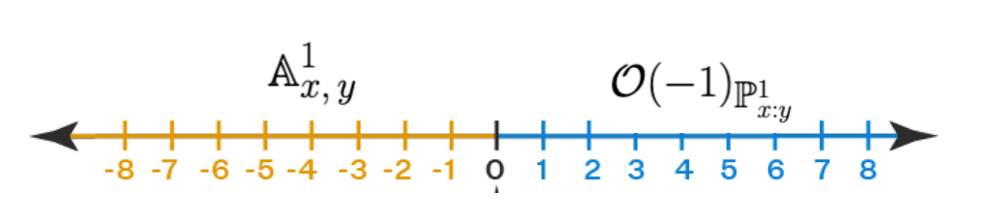
\includegraphics[width=8cm]{git/diffquotients.png}
    \caption{Secondary fan of GIT problem $\mathbb{C}^3_{(1, \, 1, \, -1 )}$}
  \end{figure}  
\end{example}
Given the weights $q_i \in L^v$ we can also define weight map $Q : \Z^n \to L^v$ in the obvious way, and we consider the kernel $A : M \to \Z^n$ of $Q$. We assume that our weight map is surjective up to torsion, so that our GIT quotient stacks do not have infinite isotropy groups. By definition $A$ is injective and by the assumption on $Q$, $M \cong \Z^{n-r}$. We call $a_i \defeq A^v(e_i) \in M^v $ \textit{rays}. We package this information in the complex
$$
0 \xrightarrow[]{} M \xrightarrow[]{A} \Z^n \xrightarrow[]{Q} L^v \xrightarrow[]{} 0
$$
Just as we cansee $Q$ as an $r\times n$ dimensional matrix, we will see $A$ as a $n \times (n-r)$ dimensional matrix.  We will often give our GIT problems as packaged in a complex, as this notation makes it easier for us to define other GIT problems using data from our original GIT problem. We will discuss this more in Section \ref{wallcrossing}.
\subsection{Wall-Crossing Formula}
\label{wallcrossing}
Let us consider a rank $r$ torus $T$ acting on a $n$-dimensional vector space $V$, with GIT problem given by complex
$$
0 \xrightarrow[]{} M \xrightarrow[]{A} \Z^n \xrightarrow[]{Q} L^v \xrightarrow[]{} 0.
$$
In \cite{derivedgit}, Daniel Halpern-Leistner relates the derived categories of GIT quotients to the equivariant derived category\footnote{This is just the derived category of $T$-equivariant coherent sheaves on $V$. } $D^b_T(V)$. In particular, given any reductive GIT problem and choice of stability condition $\theta$, he proves the existence of a \textit{semi-orthogonal decomposition}\footnote{A semi-orthogonal decomposition of a triangulated category $\mathcal{T}$ is a decomposition of $\mathcal{T}$ into triangulated subcategories $$
\mathcal{T} = \langle \mathcal{T}_1, \dots, \mathcal{T}_n \rangle
$$
such that the categories together generate $\mathcal{T}$ under shifting (think of shifting chain complexes) and taking mapping cones \cite[Chapter 1]{huybrechts}. } (SOD) of the equivariant derived category where one of the components is equivalent to $D^b(X_{\theta})$. In the case of toric GIT we can take this further and explicitly relate the derived categories of GIT quotients separated by a wall. \\
\newline
By analysing \cite{derivedgit} in the toric case, we see that given a toric GIT quotient $X_{\theta}$ we can find a finite collection $\mathcal{W}_\theta$ of $T$-equivariant line bundles\footnote{$T$-equivariant coherent sheaves on $V$ are just graded modules of the graded polynomial ring $R$ (the ring of regular functions on $V$), where the $\Z^r$ grading on $R$ is given by the action of $T$.} on $V$ and infinite collection $\mathcal{C}$ of $T$-equivariant sheaves supported on the unstable locus $S_{\theta}$ such that
\begin{enumerate}
    \item $\mathcal{W}_\theta$ and $\mathcal{C}$ generate (under shifts and cones) $D^b_T(V)$,
    \item The triangulated category generated (under shifts and cones) by $\mathcal{W}_{\theta}$ is equivalent to $D^b(X_\theta)$.
\end{enumerate}
We call $\mathcal{W}_\theta$ a \textit{window}. We emphasis that the choice of $\mathcal{W}_{\theta}$ is not unique, in particular we can always twist a window by an equivariant line bundle. Moreover, given two stability condition $\theta$ and $\phi$ separated by a wall $W$, we can find a countable infinite collection of windows $\mathcal{W}_{\theta}$ and $\mathcal{W}_{\phi}$ such that (say) $\mathcal{W}_{\phi} \subset \mathcal{W}_{\theta} $, and each of these gives us a semi-orthogonal decomposition (ignoring ordering)
\begin{equation}
\label{wallcrossingformula}
D^b(X_{\theta}) = \langle D^b(X_{\phi}), D^b(Z),\dots, D^b(Z)\rangle_{\text{SOD}}
\end{equation}
where $Z$ is constructed by a `sub-GIT problem' called a \textit{Higgs GIT problem}, which we will explain shortly, and the number of copies of $Z$ can be easily computed combinatorially. We will refer to equation \eqref{wallcrossingformula} as the \textit{wall crossing formula}. \\
\newline
The number of copies of $D^b(Z)$ is 
\begin{equation}
    \label{wcmult}
    \kappa = (\text{det} V) (\lambda_W),
\end{equation}
where $\text{det} V\defeq q_1 + \dots +q_n \in L^v$ is called the \textit{character}, and $\lambda_W \in L$ is the one-parameter subgroup perpendicular to the wall, oriented so that $\kappa \geq 0$. The GIT chamber the oriented $\lambda_W$ points to will be the maximal one (the one with the bigger derived category, i.e. $X_{\theta}$). 
\begin{definition}
Consider a subset $\mathcal{T} \subset \{1,...,n \}$ and consider the corresponding set of weights $Q(\mathcal{T})$. We define $L_{\mathcal{T}}^v$ as the primitive sublattice generated by these weights
$$L_{\mathcal{T}}^v= L^v \cap \langle  Q(\mathcal{T}) \rangle_{\mathbb{R}} \subset L_{\mathbb{R}}^v.
$$
We define a GIT problem
$$
0 \xrightarrow[]{} M_{\mathcal{T}} \xrightarrow[]{A_{\mathcal{T}}} \Z^\mathcal{T} \xrightarrow[]{Q_{\mathcal{T}}} L^v_{\mathcal{T}} \xrightarrow[]{} 0,
$$
which we call \textit{Higgs GIT problem} associated to $\mathcal{T}$.
\end{definition}
We have a Higgs GIT problem associated to a wall $W$ by taking the subset of weights to be the weights lying on the subspace spanned by the wall. We denote this subset of weights $Q(W)$, and the GIT problem as $Q_W$. This gives a rank $r-1$, dimension $|Q(W)|$ toric GIT problem. $Z$ is a GIT quotient of this new GIT problem, where we choose the stability condition to be on the wall $W$. In fact, $Z$ is a quotient of the fixed locus of the action of $\lambda_W$ by the rest of the action of $T$.
\subsection{Spherical Functors}
\label{CY}

The goal of this section will be to construct \textit{spherical functors} from the data of a toric \textit{Calabi-Yau} GIT problem. We start first by explaining some general theory about them. 
\subsubsection*{General Theory}
The first type of spherical functors that were studied were \textit{spherical objects}. Let $X$ be a smooth projective variety over a field $k$.
\begin{definition}\cite[Chapter 8]{huybrechts}
    \label{sphericalobject}
    An object $\Es^{\bullet} \in D^b(X)$ is called \textit{spherical} if 
    \begin{enumerate}
        \item $\Es^{\bullet} \otimes \omega_X \cong \Es^{\bullet}$ and,
        \item \[
        \text{Hom}_{D^b(X)}(\Es^{\bullet},\Es^{\bullet}[i]) \cong 
        \begin{cases}
            k & \text{if } i = 0, \text{dim}(X), \\
            0 & \text{otherwise}.
        \end{cases}
        \]
    \end{enumerate}
\end{definition}
These objects are called spherical because condition $(2)$ can be rephrased
$$
\text{Hom}_{D^b(X)}(\Es^{\bullet},\Es^{\bullet}[*]) \cong H^*(S^{\text{dim}(X)},k)
$$
where $S^{\text{dim}(X)}$ denotes the $\text{dim}(X)$-dimensional sphere. We define the \textit{spherical twist} $T_{\Es^{\bullet}} : D^b(X) \to D^b(X)$ about a spherical object to be 
\begin{equation}
    \label{sphericalobjecttwist}
    T_{\Es^{\bullet}} (\Fs^{\bullet}) = C\left( \text{Hom}(\Es^{\bullet}, \Fs^{\bullet})\otimes \Es^{\bullet} \xrightarrow{} \Fs\right)
\end{equation}
where the map is given by evaluation and note all the functors are derived\footnote{There are some technical issues with the definition of the spherical twist because taking cones is not functorial. We bypass any such issues because in our geometric context, where our triangulated category is the derived category of an algebraic variety, we can actually describe any spherical twist (even about a spherical functor) as a Fourier Mukai transform.}. By \cite[Proposition 8.6]{huybrechts}, the spherical twist $T_{\Es^{\bullet}}:D^b(X) \to D^b(X)$ about any spherical object $\Es^{\bullet}\in D^b(X)$ is an autoequivalence. The formula for the spherical twist may look familiar, and this is because at the level of $K$-theory it acts as reflection through the hyperplane orthogonal to the Mukai vector $v(\Es^{\bullet})$. So in a sense the spherical twist is a categorification of reflection. \\
\newline
Spherical twists about \textit{spherical functors} are generalisations of spherical twists about spherical objects. Our main reference for spherical functors is \cite[Section 1]{spherical}. Consider an exact functor $F : \mathcal{A} \to \mathcal{B}$ between triangulated categories $\mathcal{A}$ and $\mathcal{B}$. with left and right adjoints $L, R : \mathcal{B} \to \mathcal{A}$. We define the \textit{twist} $T : \mathcal{B} \to \mathcal{B}$ to be the cone on the counit $FR \xrightarrow[]{\epsilon} \text{id}_\mathcal{B}$ of the adjuction, so that there is an exact triangle 
\begin{equation}
     FR \xrightarrow[]{\epsilon} \text{id}_\mathcal{B}\xrightarrow{} T,
\end{equation}  
and the \textit{cotwist} 
\begin{equation}
    \text{id}_\mathcal{A} \xrightarrow[]{\eta}  RF \xrightarrow{} C,
\end{equation}  
We say that $F$ is spherical if $C$ is an
equivalence and $R \cong C_T L$. 
\begin{thm}[Rouquier and Anno]
    The spherical twist $T_F : \mathcal{B} \to \mathcal{B}$ about a spherical functor $F : \mathcal{A} \to \mathcal{B}$ is an autoequivalence.
\end{thm}
\begin{proof}
    Though attributed to Rouquier and Anno, Nick Addington gives a proof \cite[Theorem 1]{spherical}. 
\end{proof}
How is a spherical twist about a spherical functor a generalisation of the spherical twist about a spherical object? Suppose we have a spherical object $\Es^{\bullet} \in D^b(X)$ with $X$ a smooth projective variety over $k$. We define:
$$
F = \Es^{\bullet} \otimes - : D^b(pt) \xrightarrow{} D^b(X).
$$
We can prove that $F$ is a spherical functor, and since $R = \text{RHom}(\Es^{\bullet}, -)$, the twist $T_F : D^b(X) \to D^b(X)$ is exactly like the twist $T_{\Es^{\bullet}}$ we defined earlier. Note that $R \cong C_T L$ just amounts to condition (1) in Definition \ref{sphericalobject}.


\subsubsection*{Spherical functors in toric CY GIT}
Let us consider a rank $r$ torus $T$ acting on a $n$-dimensional vector space $V$. Let $X$ and $X'$ be two GIT quotients separated by a wall $W$. In this subsection we will be defining a spherical functor $F : D^b(Z) \to D^b(X) $ for \textit{Calabi-Yau} toric GIT problems, where $Z$ is the same variety showing up in the wall-crossing formula \eqref{wallcrossingformula}. Note that in \cite{gitauto}, Halpern-Leistner and Shipman proved that the autoequivalences coming from wall crossing give the autoequivalences coming from these spherical functors. \\
\newline
We start by explaining what we mean by a Calabi-Yau toric GIT problem. Our GIT problem is given by a complex
$$
0 \xrightarrow[]{} M \xrightarrow[]{A} \Z^n \xrightarrow[]{Q} L^v \xrightarrow[]{} 0.
$$
\begin{definition}
    We say a torus action $T$ on $V$ is \textit{Calabi-Yau} if $T$ acts through $SL(V)$.
\end{definition}
If $T$ acts through $SL(V)$, then for all $(\lambda_1, \dots, \lambda_r) \in (\CC^*)^r$, we require the matrix by which the torus acts 
$$
\begin{pmatrix}
{\lambda_1}^{q_{11}}{\lambda_2}^{q_{21}}\dots {\lambda_r}^{q_{r1}} & 0 & \cdots & 0 \\
0 & {\lambda_1}^{q_{12}}{\lambda_2}^{q_{22}}\dots {\lambda_r}^{q_{r2}} & \cdots & 0 \\
\vdots & \vdots &  \ddots & \vdots \\
0 & 0 & \dots & {\lambda_1}^{q_{1n}}{\lambda_2}^{q_{2n}}\dots {\lambda_r}^{q_{rn}}
\end{pmatrix}
$$
to have determinant 1. This means
$$
{\lambda_1}^{q_{11} + \dots + q_{1n}} {\lambda_2}^{q_{21} + \dots + q_{2n}}
\dots {\lambda_r}^{q_{r1} + \dots + q_{rn}} = 1
$$
for all $\lambda_i \in \CC^*$. So we need the sums $q_{m1} + \dots + q_{mn} = 0$ for all $m \in \{1, \dots, r \}$, in other words we need the sum of the entries in each row of our weight matrix $Q$ to be 0. We call this the Calabi-Yau case, because our GIT quotients are Calabi-Yau if and only if the torus acts through $SL(V)$.\\
\newline
Let us consider a wall $W$ in our GIT problem. Because of the Calabi-Yau condition, the number of copies of $D^b(Z)$ in the wall crossing formula is 0. This is because $\text{det}V=0$ in formula \eqref{wcmult}. We instead use the wall-crossing formula on $D^b(Z)$ itself in the Higgs problem $Q_W$, which may not be Calabi-Yau. Upon applying the wall crossing formula once we find
$$
D^b(Z) = \langle D^b(Z'), D^b(Y),...,D^b(Y) \rangle_{SOD},
$$
where $Z'$ is a GIT quotient in $Q_W$ that's separated by a wall $W'$ from $Z$, and $Y$ is a subvariety coming from a the Higgs GIT problem of $Q_W$ associated to $W'$. Notice this GIT problem will also be a Higgs GIT problem of our original GIT problem $Q$. We imagine iterating the wall crossing formula on $D^b(Z')$ and $D^b(Y)$ until we can no longer cross to a more minimal quotient. This always terminates after a finite number of steps as each step strictly decreases the rank of the GIT problems. We get SOD (ignoring ordering):
\begin{equation}
    \label{Zsod}
    D^b(Z) = \langle D^b(Z_0), \dots, D^b(Z_0), \dots, D^b(Z_k), \dots D^b(Z_k)\rangle_{SOD}
\end{equation}
where each $Z_i$ is a minimal GIT quotient for a Higgs problem of our original GIT problem. In \cite{kite2022discriminants} Kite-Segal prove that no matter how we choose to wall-cross, the subcategories occurring in the final decomposition and their multiplicities are independent of all choices. In the same paper, they show that the irreducible factors $Z_i$ come from Higgs problems associated to \textit{relevant subspaces}.
\begin{definition}
    We call a subspace $H \subset L_{\mathbb{R}}^v$ \textit{relevant} if the cone spanned by the weights lying in $H$ is the whole of $H$.
\end{definition}
A relevant subspace $H$ defines a Higgs GIT problem by considering the weights lying on $H$. These Higgs GIT problems will have a non-empty minimal phase $Z_H$. The important point is that $Z_H$ are precisely the factors $Z_0, \dots, Z_k$ in the SOD \eqref{Zsod} for $D^b(Z)$. In other words, the relevant subspaces $H$ index the irreducible factors.  \\
\newline
So how is the spherical functor $F$ defined? In Section \ref{GIT} we presented a method to analyse the stability of points in a toric GIT problem. An equivalent and more general method is the \textit{Hilbert-Mumford Criterion}, which essentially says it's enough to analyse the stability of points in the GIT problems coming from one-parameter subgroups \cite{mumford}. A point will then be (semi-)stable if it is (semi-)stable for all one-parameter subgroups. In practice in toric GIT problems we only need to consider a finite number of one-parameter subgroups. \\
\newline
We now note that the stability condition for $X$ and $X'$ only differ by one parameter subgroup $\lambda_W$ normal to the wall. This means only one irreducible component of the unstable for points will different. We look at the component that we remove to obtain $X'$ and see it as a subset of $X$. We denote it $Y$. $Y$ is a bundle over $Z$ by \cite{bialynick} so we have maps
\begin{center}
\begin{tikzcd}
  Y \arrow[d,"\pi"] \arrow[r, "i"] & X \\
  Z &
\end{tikzcd}
\end{center}
and $F \defeq i_* \pi^*$ where all of the functors are derived. Note the right adjoint is $R = \pi_* i^!$. \\
\newline
Recall that the wall-crossing algorithm produced a semi-orthogonal decomposition:
$$D^b(Z) =\langle \mathcal{C}_1,...,\mathcal{C}_m\rangle $$
By Theorem 4.14 in \cite{gitauto}:
\begin{enumerate}
    \item The restriction of $F$ to each piece gives a spherical functor $F_i : \mathcal{C}_i \to D^b(X)$, where we mean restriction in the sense of \cite[Chapter 1]{huybrechts},
    \item The spherical twist $T_F$ factors as:
    \begin{equation}
        \label{twistfactors}
        T_F = T_{F_1} \circ \dots \circ T_{F_m},
    \end{equation}
\end{enumerate}
So for each wall and relevant subspace $H$, we get some spherical functors $F_H :D^b(Z_H) \to D^b(X)$.\\
\newline
In the next section we discuss how to construct the $FIPS$ and in particular describe the discriminant locus $\Delta$. The $FIPS$ will be the complement of $\Delta$, and the upshot is that $\Delta$ decomposes into a union of discriminant loci 
$$
\Delta = \bigcup_{i=0}^k \Delta_i,
$$
and each such component will correspond to a variety $Z_i$ from the SOD \eqref{Zsod}. In our conjecture we will therefore want meridians in $\Pi_1(FIPS)$ about $\Delta_i$ to act by twists by spherical functors $F_i :D^b(Z_i) \to D^b(X)$.

\subsection{FIPS}
\label{fips}
Let us consider a rank $r$ torus $T$ acting on a $n$-dimensional vector space $V$, with GIT problem given by complex
$$
0 \xrightarrow[]{} M \xrightarrow[]{A} \Z^n \xrightarrow[]{Q} L^v \xrightarrow[]{} 0.
$$ 

If we choose a basis for $M$, $A$ is represented by $n\times (n-r)$ dimensional integer matrix. Let $P \in \Z^k \otimes_{\Z} \R$ be the convex hull of the rays $a_i = A^T(e_i) \in \Z^{n-r}$. We call $P$ the primary polytope. Since we could have chosen a different basis for $M$, we have an action by $GL_k(\Z)$ on this polytope. If we assume the Calabi-Yau condition, we can choose a basis for $M$ so that the column of $A$ is a list of 1s. This shows that the primary polytope $P$ lives at height 1 and  is $k-1$ dimensional.  The different triangulations of the primary polytope correspond precisely to the different GIT quotients, in that the cone on the triangulated polytope gives you the toric fan of your quotient. \\
\newline
The \textit{superpotential} $W_{a}$ associated to our GIT problem is the Laurent Polynomial with Newton Polytope given by the rows of $A$. Explicitly, we assign independent variables $X_1,...,X_{n-r}$ to each column and for each row of $A$ we consider the monomial in $X_1,...,X_{n-r}$ given by the entries of $A$ in that row. The \textit{superpotential} $W_{a}$ associated to our GIT problem is a linear combination of these monomials:
\begin{equation}
    \label{superpotential}
    W_a(X_1,\dots,X_{n-r}) = \sum_{i=1}^n a_i\prod_{j=1}^{n-r}X_j^{A_{ij}}
\end{equation}
Landau Ginzburg models $((\CC^*)^{n-r},W_a)$, where we see the coefficients $a \in (\CC^*)^{n}$ as being fixed, are Hori-Vafa mirrors to our GIT problem \cite{horivafa}. Not all coefficients $a \in (\CC^*)^{n}$ give a mirror though. There are non-generic coefficients for which $W_a$ does not give a mirror. These non-generic coefficients live on a hypersurface called \textit{the discriminant locus} of $W_a$. Recall the discriminant for polynomials in one variable (say quadratics or cubics) captures the non-generic behaviour of having roots with multiplicity greater than 1. The discriminant locus we refer to is a generalisation of this discriminant but for any Laurent polynomial in any number of variables. The theory for this generalised discriminant locus can be found in book \cite{gelfand1994discriminants} by Gelfand-Kapranov-Zelevinski. For this reason the discriminant locus is sometimes referred to as the GKZ discriminant locus. \\
\newline
The discriminant locus $\Delta$ of $W_a$ decomposes into a union of other irreducible discriminant loci:
$$
\Delta = \bigcup_{i=0}^k \Delta_i,
$$
and we will start by explaining how to compute the \textit{principal discriminant component}, which is one of our discriminant components $\Delta_i$. We consider the non-generic $a$:
$$
D_A= \{ a \in (\CC^*)^n \: | \: \exists x \in(\CC^*)^{n-r} \text{ such that $W_a(x) =0$ and $dW_a(x) =0.$} \}
$$
The closure of $D_A$ is an affine variety, which is always irreducible \cite[Ch. 9]{gelfand1994discriminants}. In nice examples we can directly compute $D_A$ by solving the system of equations, however in generality this will not work. For example, even the discriminant of the cubic requires more work to deduce. There is a method which in principle allows one to always compute $D_A$ called \textit{The Cayley Method} \cite[Ch. 2]{gelfand1994discriminants}, although it quickly becomes computationally involved. In the interest of brevity we won't explain the details of it in this report, so we will restrict ourselves to examples where the computation is straight-forward.\\
\newline
We note that $D_A$ is invariant under a rank $n-r$ torus action with weight map $A^v$ (in matrix form this is just taking the transpose). This follows because $D_A$ is invariant under rescaling the $X_i$ variables and an action by $A^v$ on the coefficients $a \in (\CC^*))^{n}$ can be absorbed by the variables by rescaling. We can hence quotient $D_A \subset (\CC^*)^n$ by $(\CC^*)^{n-r}$ and get $\Delta_A \subset (\CC^*)^r$. We call $\Delta_A$ the \textit{principal discriminant} of $A$. Note we did not have to use GIT theory when we took the quotient here as the action is free and hence the naive topological quotient is geometric. \\
\newline
What about the other discriminant components? If we pick a subset $\mathcal{S} \subset \{1, \dots, n \}$, we can consider the collection of rows of $A$ corresponding to $\mathcal{S}$. We write $A^{\mathcal{S}}$ for the matrix which is the collection of such rows. We define the discriminant component $\Delta_{\mathcal{S}}$ associated to $\mathcal{S}$ to be essentially the principal discriminant component of $A^{\mathcal{S}}$ and see it as living $(\CC^*)^r$ by seeing $D_{A^{\mathcal{S}}}$ as living in $(\CC^*)^{|\mathcal{S}|} \subset (\CC^*)^{n} $. The discriminant locus will be a union of these discriminants $\Delta_{\mathcal{S}}$ for some $\mathcal{S}$. Note $\Delta_A = \Delta_{\{1,\dots,n \}}$. We compute an example below to make this all clear.
\begin{example}
    \label{exmpdisc}
    \label{components}
    Consider GIT problem 
    $$
    0 \xrightarrow[]{} \Z^3 \xrightarrow[]{A} \Z^4 \xrightarrow[]{Q} \Z \xrightarrow[]{} 0.
    $$
    with
    $$
    Q = 
    \begin{pmatrix}
        2 & -1 & -1 & 0
    \end{pmatrix},
    \hspace{0.5cm}
    A =
    \begin{pmatrix}
        1 & 0 & 0 \\
        1 & 0 & 1 \\
        1 & 0 & -1 \\
        1 & 1 & 0
    \end{pmatrix}
    \begin{matrix}
        a \\
        b \\
        c \\
        d
    \end{matrix}
    $$
    We assign independent variables $X,Y$ and $Z$ to the columns of $A$ in order. By definition \eqref{superpotential}, we have superpotential
    \begin{align*}
    W_{a,b,c,d}(X,Y,Z) &= aX + b XZ + c X Z^{-1} + dXY,\\
                        & = X(a + bZ + c Z^{-1} + dY).
    \end{align*}
    We compute partial differentials
    \begin{align}
        \frac{\partial W_{a,b,c,d}}{\partial X} &= a + bZ +cZ^{-1} + dY, \\
        \label{eqn0}
        \frac{\partial W_{a,b,c,d}}{\partial Y} &=dX, \\
        \frac{\partial W_{a,b,c,d}}{\partial Z} &= X(b - cZ^{-2}).
    \end{align}
    There is no $X \in \CC^*$ for which \eqref{eqn0}=0, so the principal discriminant locus is empty. Consider $\mathcal{S} = \{1,2,3 \}$. We have 
    $$
    A^{\mathcal{S}} =
    \begin{pmatrix}
        1 & 0 & 0  \\
        1 & 0 & 1  \\
        1 & 0 & -1 
    \end{pmatrix}
    $$.
    We have associated superpotential and differentials
    \begin{align}
        W_{a,b,c}^{\mathcal{S}}(X,Y,Z)  &= X(a + bZ + c Z^{-1} ), 
        \nonumber \\
        \label{eqn2}
        \frac{\partial W_{a,b,c,d}^{\mathcal{S}}}{\partial X} &= a + bZ +cZ^{-1}, \\
        \frac{\partial W_{a,b,c,d}^{\mathcal{S}}}{\partial Y} &=0, \\
        \label{eqn4}
        \frac{\partial W_{a,b,c,d}^{\mathcal{S}}}{\partial Z} &= X(b - cZ^{-2}).
    \end{align}
    \eqref{eqn4}=0 implies $Z = \pm \sqrt{\frac{c}{b}}$. Plugging this into \eqref{eqn2}=0 we find $D_{A^{\mathcal{S}}} = \{a^2 = 4 cb \}\subset (\CC^*)^{4}_{a,b,c,d}$. We can use the rank 3 torus action to scale out $a$, $c$, and $d$ and we get discriminant component $\{c=1/4 \} \in \CC^*_c$. We haven't shown this yet but it turns out that this gives us the only non-trivial component of the discriminant locus $\Delta$ of $A$, so that $FIPS$ is $\CC^* \backslash \{ 1/4 \} $.
\end{example}
Not all subsets $\mathcal{S}$ give us discriminant components. Only a certain type of subset will be important for us. These are the \textit{minimal faces} of our primary polytope $P$. 
\begin{definition}
    A face $\Gamma \subset P $ is called \textit{minimal} if every ray in $\Gamma$ is linearly dependent on the other rays in $\Gamma$.
\end{definition}
The only subsets $\mathcal{S}$ we care about are those that correspond to minimal faces of the primary polytope $P$. This leads us to the following definitions.
\begin{definition}
    The discriminant locus $\Delta$ is the union of the subvarieties $\Delta_{\Gamma}$, for each minimal face $\Gamma \subset P$ such that $\Delta_{\Gamma}$ is a hypersurface.
\end{definition}
\begin{definition}
    \label{FIPS}
    We define the Fayet-Iliopoulos Parameter Space ($FIPS$) to be the complement of the discriminant locus $\Delta$ in $(\CC^*)^r$.
\end{definition}
\begin{example} [Example \ref{exmpdisc} continued]
    In Example \ref{exmpdisc}, the primary polygon is as in Figure \ref{gkzcomponents} below.
    \begin{figure}[!h]
        \centering
        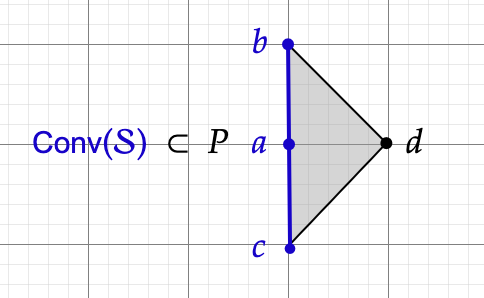
\includegraphics[width=5cm]{face&subspace/primary.png}
        \caption{The primary polygon $P$ and minimal face $\mathcal{S}$.}
        \label{gkzcomponents}
    \end{figure}
    We only have two minimal faces: the whole polygon $P$ itself and the face that is the convex hull of $\mathcal{S}$, denoted $\text{Conv}(\mathcal{S})$. This is why the principal component and the component associated to $\mathcal{S}$ gave us the entire discriminant locus.
\end{example} 
The following proposition is what allows us to relate discriminant components to components in the wall-crossing SOD \eqref{Zsod} for $Z_W$ associated to a wall $W$ in the secondary fan. We just discussed that the former components correspond to minimal faces, and we recall that the components of the latter correspond to relevant subspaces.
\begin{prop}
    \label{faces&subspaces}
    Let $\Gamma \subset P$ be a minimal face of the primary polytope and consider its indexing subset in $\{1,\dots,n \}$, which by abuse of notation we denote $\Gamma$ too. We can consider subspace $H_{\Gamma^c}$ spanned by the weights associated to the indexing subset $\Gamma^c$. $H_{\Gamma^c}$ is relevant, and moreover the map $\Gamma \to H_{\Gamma^c}$ is a bijection between the minimal faces of $P$ and the relevant subspaces of $L_{\mathbb{R}}^v$.
\end{prop}
\noindent
Proposition \ref{faces&subspaces} may inspire us to make some (possibly vague) guesses on how the fundamental group of $FIPS$ acts on the derived categories of our GIT quotients. By the correspondence, we may roughly postulate that loop around a discriminant component $\Delta_\Gamma$ should correspond to a spherical twist about a spherical functor $F_{\Gamma} : D^b(Z_{\Gamma^c}) \to D^b(X)$. \\
\newline
Let us first describe an insightful way to think about $FIPS$. Since $FIP=(\CC^*)^r \backslash \Delta $, we can see $FIPS$ as living inside the secondary toric variety $\Fs$, which is $r$-dimensional too. It turns out that the secondary toric variety is a particularly nice compactification of $FIPS$. We can compactify the discriminant locus $\bar{\Delta} $ in $\Fs$ and we see $FIPS$ now as $\Fs \backslash \bar{\Delta} \cup \{\text{toric boundary} \}$. \\
\newline
Recall that the fixed points under the torus action in $\Fs$ correspond to GIT quotients. These clearly live in the toric boundary $\Fs \backslash (\CC^*)^r$ and hence not in $FIPS$. The toric boundary is the union of the divisors corresponding to the 1-dimensional cones in the secondary fan via orbit-cone correspondence. Suppose there are $m$ 1-dimensional cones and denote the corresponding divisors $D_i$. We can consider the fundamental groupoid of $FIP= \Fs \backslash \bar{\Delta} \cup D_1 \cup \dots \cup D_m$ with base point set being made up of one base point per GIT quotient, chosen to be `close' to the point in $\Fs$ corresponding to the GIT quotient. 
\begin{conjecture}[Main Conjecture]
    \label{main}
    Let us consider toric Calabi-Yau GIT problem $T$ acting on $V$. We consider the fundamental groupoid of $FIPS= \Fs \backslash \bar{\Delta} \cup D_1 \cup \dots \cup D_m$ with base point set being made up of one base point per GIT quotient, chosen to be `close' to the point in $\Fs$ corresponding to the GIT quotient. We denote the fundamental groupoid $\Pi_1(FIPS)$. Then $\Pi_1(FIPS)$ acts faithfully on the set $S$ of the derived categories of our GIT quotients via equivalences. Moreover this action also satisfies:
    \begin{enumerate}
        \item Given two GIT quotients $X$ and $Y$ separated by a wall and a derived equivalence through wall-crossing, there is a path in $\Pi_1(FIPS)$ that acts on $S$ via that derived equivalence.
        \item Given a GIT quotient $X$, a loop around a discriminant component $\Delta_\Gamma$ should correspond to a spherical twist about a spherical functor $F_{\Gamma} : D^b(Z_{\Gamma^c}) \to D^b(X)$.
        \item Given a GIT quotient $X$, recall that there is a corresponding chamber in the secondary fan. Then loops around the toric boundary divisors from 1-dimensional cones in the chamber correspond to twists by $\text{Pic} X$.
    \end{enumerate}
\end{conjecture}
We will be proving conditions (2) and (3) of this conjecture in a rank 2 GIT problem in Section \ref{rank2example}.
\begin{remark}[Important Remark]
\label{stacky}
We make a remark with regards to Definition \ref{FIPS} of $FIPS$. It turns out that if we want condition (3) in Conjecture \ref{main} to be true, we may need to consider a bigger class of coefficients of the superpotential $W_a$. A priori we considered $a \in (\CC^*)^{n}$, but we actually need to be more careful. If a ray (row of $A$) is not a vertex of the primary polytope $P$, then it turns out we should allow the corresponding coefficient to be 0 in $FIPS$ as otherwise we lose stacky information. So in fact we consider $a \in (\CC)^{n} \backslash \{ \prod_{a_i\in \text{Vert}P} a_i \}$. We will illustrate this in the following example.
\end{remark}
\begin{example}[Example \ref{exmpdisc} continued]
    The GIT problem in Example \ref{exmpdisc} is $\CC^*$ acting on $\CC^4$ by $\lambda \cdot (x,y,z,w) = (\lambda^2x , \lambda^{-1}y, \lambda^{-1}z,w) $. The secondary fan is
    \begin{figure}[!h]
        \centering
        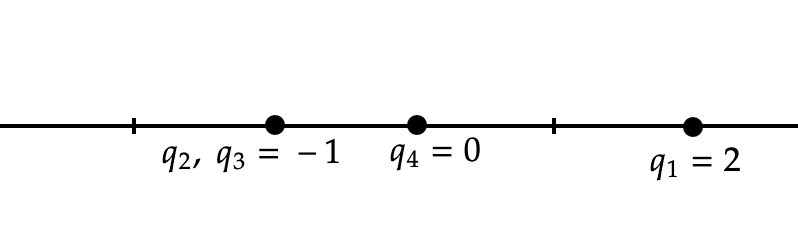
\includegraphics[width=6cm]{face&subspace/secondary.png}
        \caption{The secondary fan.}
    \end{figure}\\
    The secondary toric variety is the smooth stack $\Fs = \mathcal{P}^1_{q_1,q_2}(2,1)$. A positive stability condition will have us remove $\{ x=0\}$. We scale out the $x$ coodinate but end up with a leftover $\Z_2$ action with weight 1 on the $y$ and $z$ coordinates, so we have quotient $X_+ = [\CC^2_{y,z}/ \Z_2] \times \CC_w$. A negative stability condition will have us remove $\{ y=z=0\}$, and so we have quotient $X_- = \CC^2_{x,w} \times \PP^1_{[y:z]}$. So $\text{Pic} X_+ = \Z_2$ and $\text{Pic} X_- = \Z$.  \par
    To $\mathcal{S} = \{ 1,2,3\}$ we have corresponding relevant subspace $H_{\{4\}} =0$ via Proposition \ref{faces&subspaces}. The GIT problem for this relevant subspace is $\CC^*$ acting on $\CC$ with weight 0. The quotient is obviously just $\CC$ (with infinite istropy group though?). \par
    Recall we computed that the discriminant locus (before quotienting by the action of $A$) was $\{a^2 = 4ab \} \subset (\CC^*)^{4}_{a,b,c,d}$. Note though in Figure \ref{gkzcomponents}, $a$ is not one of the vertices of the primary polytope. By Remark \ref{stacky}, $FIPS$ should actually be the complement of $\{a^2 = 4ab \}$ in $\CC_a \times (\CC^*)^3_{b,c,d}$ instead. We use $A$ to scale out $b,c,d$ and  we end up with a $\Z_2$ action on $a$, so $FIPS = [\CC_a \backslash \{a = \pm 2 \} / \Z_2 ]$. We see $FIPS$ as a subset of $\Fs$ via embedding $a \mapsto [a:1]$. $[0:1]$ in $\Fs$ corresponds to $X_+$, which corresponds to the origin in $FIPS$. If we pick base point in $FIPS$ close to 0 we get orbifold fundamental group $ \pi_1(FIPS) = \langle \alpha, \beta | \alpha^2, [\alpha,\beta] \rangle$ where $\alpha$ corresponds to a loop around the origin and $\beta$ is a loop around $a = \pm 2$. $\pi_1(FIPS)$ should act on $D^b(X_+)$ where $\alpha$ is twisting by the generator of $\text{Pic} X_+ = \Z_2$ and $\beta$ is the spherical twist about spherical functor $F : D^b(\CC_w) \to D^b(X_+)$ given by inclusion. Note that if we didn't have relation $\alpha^2$ in $\pi_1(FIPS)$ this wouldn't work, which is why Remark \ref{stacky} is important.
\end{example}


\section{Rank 2 Example}  
\label{rank2example}
Let us consider rank 2 toric GIT problem $(\CC^*)^2$ acting on $\CC^5$ via weight matrix $Q : \Z^5 \to \Z^2$:
\begin{align*}
    Q =& \begin{pmatrix}
    -2 & 1 & 1 & 0 & 0 \\
    -2 & 0 & 0 & 1 & 1
    \end{pmatrix} 
    \\
    & \hspace{0.7cm}\begin{matrix}
    a & b & c & d & e 
    \end{matrix}
\end{align*}
We have kernel $A : \Z^3 \to \Z^5$:
\begin{equation*}
    A = 
    \begin{pmatrix}
    1 & 0 & 0 \\
    1 & 1 & 0 \\
    1 & -1 & 0 \\
    1 & 0 & 1 \\
    1 & 0 & -1
    \end{pmatrix}
    \:
    \begin{matrix}
    a \\
    b \\
    c \\
    d\\
    e
    \end{matrix}
\end{equation*}
We start by computing what our GIT quotients are. It turns out when the character lattice is 2-dimensional, the wall and chamber decomposition described in Section \ref{GIT} is produced immediately by taking the positive cones on the weights. 
\begin{figure}[!h]
    \centering
    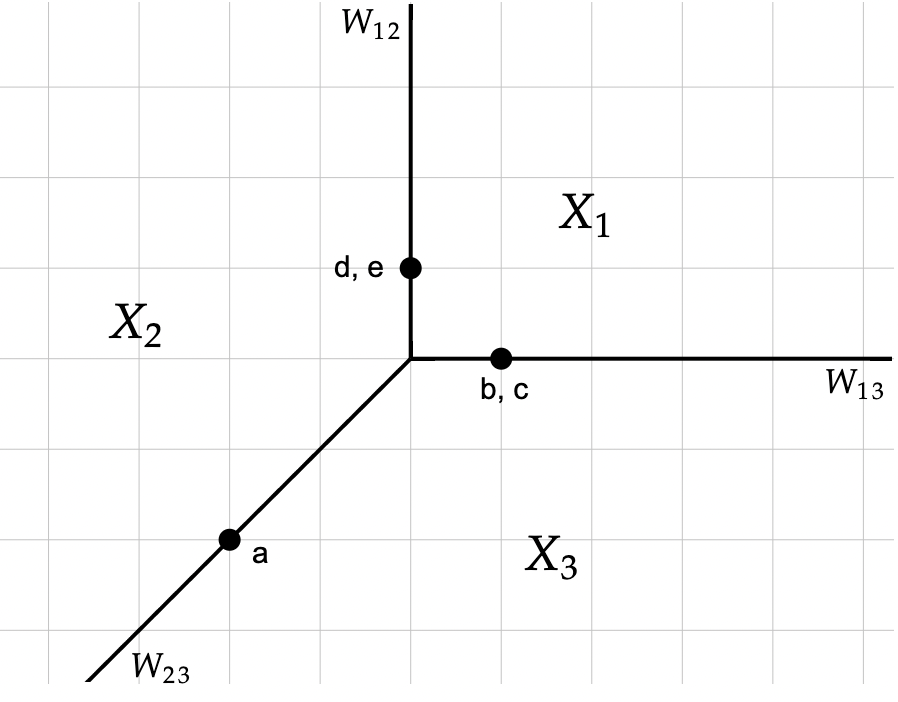
\includegraphics[width=8cm]{rank2exmp/secondaryfan1.png}
    \caption{The secondary fan of the rank 2 example.}
    \label{secondaryrank2}
\end{figure}\\
\newline
In Figure \ref{secondaryrank2}, labelled by $X_1, X_2$ and $X_3$, and between them, walls $W_{12}$, $W_{13}$, and $W_{23}$. As per Section \ref{GIT} we compute the ideals:
\begin{align*}
    \mathcal{I}_{X_1} &= \langle db, dc, eb, ec \rangle \\
    \mathcal{I}_{X_2} &= \langle da, ea \rangle \\
    \mathcal{I}_{X_3} &= \langle ba, ca \rangle
\end{align*}
Using toric geometric invariant theory we get that the unstable loci for each chamber $X_i$ is given by the vanishing of the ideal $ \mathcal{I}_{X_i}$
\begin{align*}
    S_1 &= V(\mathcal{I}_{X_1}) = \{  d= e= 0\} \cup \{ b=c=0\} \\
    S_2 &= V(\mathcal{I}_{X_2}) = \{ a= 0 \} \cup \{ d = e= 0\} \\
    S_3 &= V(\mathcal{I}_{X_3}) = \{ a= 0 \} \cup \{  b= c= 0\}
\end{align*}
and so our GIT quotients are
\begin{align*}
    X_1 &= \frac{\CC^5 \backslash \{  d= e= 0\} \cup \{ b=c=0\} }{ (\CC^*)^2}\\
    X_2 &= \frac{\CC^5 \backslash \{  a= 0\} \cup \{ d = e= 0\} }{ (\CC^*)^2} \\
    X_3 &= \frac{\CC^5 \backslash \{ a= 0 \} \cup \{  b= c= 0\} }{ (\CC^*)^2}
\end{align*}
It's not hard to see that our quotients are in fact the smooth Deligne-Mumford stacks
\begin{align*}
    X_1 &= {\mathcal{O} (-2, -2)}_{\PP^1_{b:c} \times \PP^1_{d:e}} \\
    X_2 &= \left[{\mathcal{O}(-1)^{\oplus 2}}_{\PP^1_{d:e}} / \Z_2 \right] \\
    X_3 &= \left[{\mathcal{O}(-1)^{\oplus 2}}_{\PP^1_{b:c}} / \Z_2 \right]
\end{align*}
where $\Z_2$ acts on the fibres by $-1$ for both $X_2$ and $X_3$, so that we have a stacky $\PP^1$ in both cases (the zero sections of the rank 2 vector bundles). \\
\newline
\noindent
We can also look at the primary polytope $P \subset \Z^2$, which in this case is just a polygon. Recall that triangulations of the $P$ give us toric fans for our GIT quotients, see Figure \ref{fig:primary}. For a detailed explanation of how to find which triangulation corresponds to which chamber, see Section 4 of \cite{coates2018crepant}.
\begin{figure}[!h]
\centering
\begin{subfigure}{.5\textwidth}
  \centering
  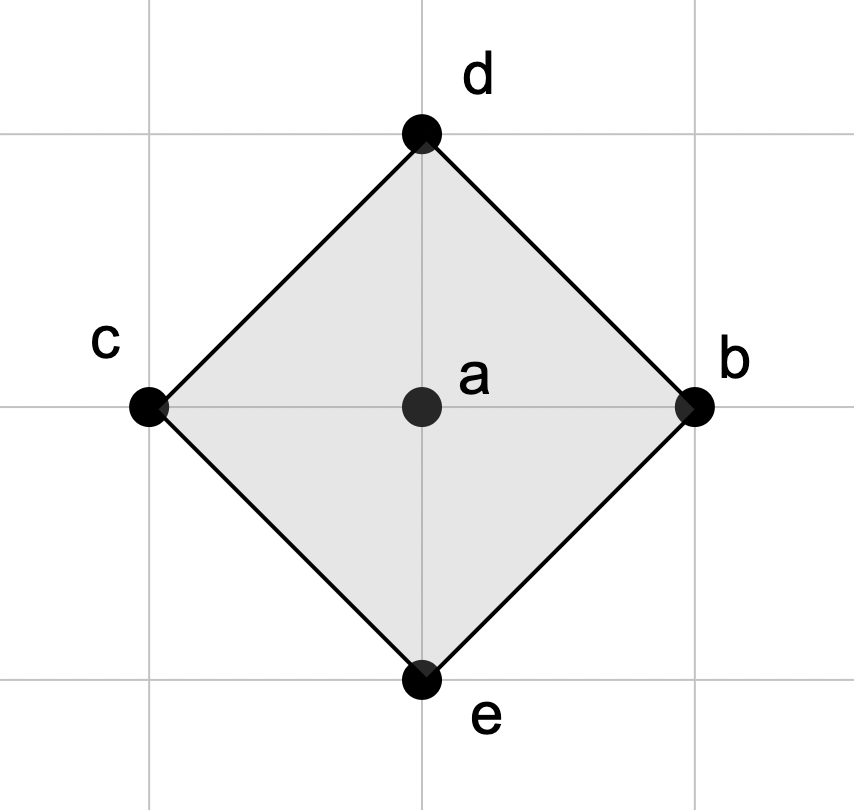
\includegraphics[width=.8\linewidth]{rank2exmp/primarypolygon1.png}
  \caption{The primary polytope.}
  \label{fig:primary}
\end{subfigure}%
\begin{subfigure}{.5\textwidth}
  \centering
  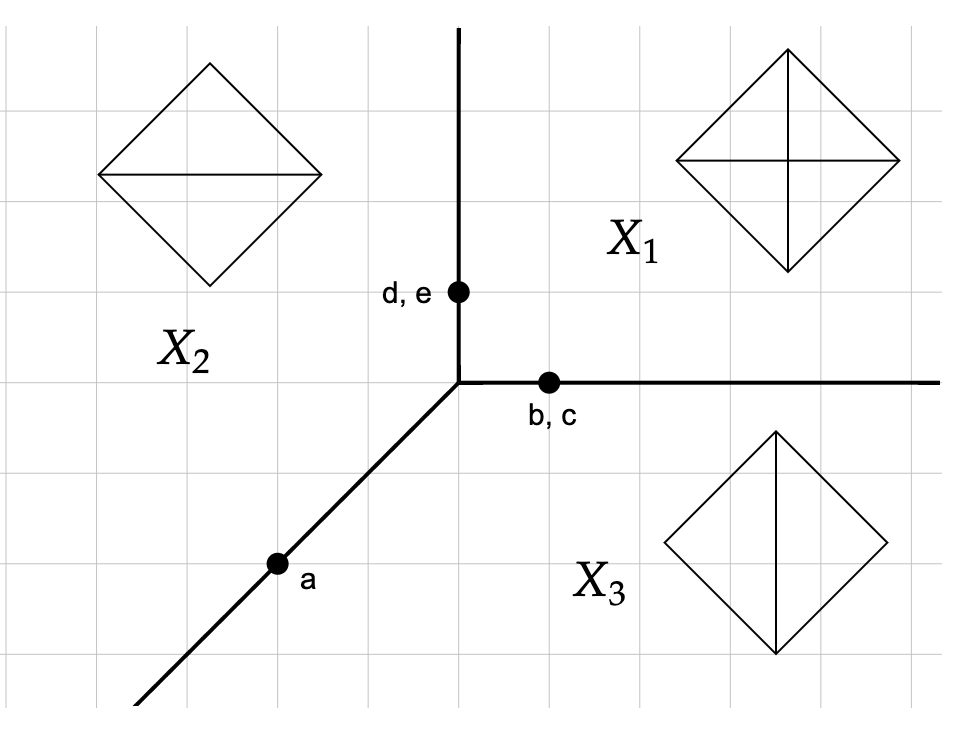
\includegraphics[width=.8\linewidth]{rank2exmp/toricfans1.png}
  \caption{The secondary polytope with the triangulations of the primary polygon. }
  \label{fig:sub2}
\end{subfigure}
\caption{}
\label{fig:test}
\end{figure}
By Section \ref{fips}, we have only one discriminant component, the principal one, because our $P$ has no minimal faces other than $P$ itself. So $\Delta = \Delta_P$. We compute the non-generic coefficients of the Laurent polynomial $W_{a,b,c,d,e} : (\CC^*)^3 \to \CC$
\begin{equation*}
    W_{a,b,c,d,e}(X,Y,Z) = X\left(a + bY + cY^{-1} + d Z + e Z^{-1}\right)
\end{equation*}
where $(a,b,c,d,e) \in \CC^5 \backslash \{ bcde = 0\}$. Note we don't remove $\{a=0 \}$ as the corresponding ray in Figure \ref{fig:primary} of the primary polytope $P$ is not a vertex of $P$. Non-generic coefficients $D_A$ of $W_{a,b,c,d,e}$ are $(a,b,c,d,e) \in \CC^5 \backslash \{ bcde = 0\}$ where $W_{a,b,c,d,e}$ has critical values. By construction we have an action of the 3-dimensional torus $(\CC^*)^3$ on $\CC^5 \backslash \{ bcdeD_A = 0\}$ with weights prescribed by the matrix $A^T$. We quotient by $(\CC^*)^3$ and get that our $FIPS$ is the smooth DM stack
$$
FIPS = \mathcal{P}^2_{1:2:2}\backslash \{bd\Delta = 0\}
$$
where we scaled $c$ and $e$ to 1 and are in coordinates $[a:b:d]$, and $\Delta$ is the image of $D_A$ after quotienting. \\
\newline
The secondary toric stacky fan is $\mathcal{F} = (\Z^2, \Sigma_{\PP^2},\beta : \Z^3 \to \Z^2)$ where $\Sigma_{\PP^2}$ is the standard toric fan for $\PP^2$, and $\beta$ is given by
$$
\beta(e_1)= (-2,-2), \: \beta(e_2) = (1,0), \: \beta(e_3) = (0,1)
$$
The realisation of this stacky fan is the smooth DM stack $\mathcal{F} \defeq \PP^2_{1:2:2}$, with coordinates $[a:b:d]$. We can see directly how $FIPS$ naturally embeds into $\mathcal{F}$ via inclusion. 

\begin{comment}
Before we compute the discriminant locus, we set some expectations of what it will look like by using a conjecture on multiplicities of Kite-Segal \cite{kite2022discriminants}, which was proved by Jesse-Huang in \cite{huang2022gkz}. Using toric orbit-cone correspondence, every wall $W_{ij}$ corresponds to a curve $C_{ij}$ the secondary toric stack $\mathcal{F} = (\Z^2, \Sigma_{\PP^2},\beta : \Z^3 \to \Z^2)$ where $\Sigma_{\PP^2}$ is the standard toric fan for $\PP^2$, and $\beta$ is given by
$$
\beta(e_1)= (-2,-2), \: \beta(e_2) = (1,0), \: \beta(e_3) = (0,1)
$$
More concretely, the secondary toric stack is the smooth DM stack $\mathcal{F} \defeq \PP^2_{1:2:2}$, with coordinates $[a:b:d]$. In these coordinates, $C_{23} = \{ a= 0\}$, $C_{13} = \{b=0\}$, and $C_{12} = \{d=0\}$. We can see directly how $FIPS$ naturally embeds into $\mathcal{F}$ via inclusion. By Corollary 4.12 in \cite{kite2022discriminants}, the discriminant locus $\Delta$ intersects each $C_{ij}$ in exactly one point. It turns out that the multiplicity with which $\Delta$ intersects the boundary curves is equal to a multiplicity in the context of semi-orthogonal decompositions that arise through wall-crossing. We will explain this now.  \\
\newline
Associated to each wall $W$  we have a \textit{Higgs GIT problem}, described in Section 2.3 of \cite{kite2022discriminants}. The cone $W$ corresponds to a chamber of the Higgs GIT problem and hence we have a corresponding phase $Z$. Another way to think of $Z$ is the fixed locus in $\CC^5$ of the one parameter subgroup $\lambda_W$ normal to wall, quotiented by the remaining action. For example, for $W_{1,3}$ the fixed locus under $(0,1)$ is $a=d=e=0$, and we can quotient by the remaining action and find $Z_{1,3} = \PP^1_{b,c}$. Similarly, $Z_{12} = \PP^1_{d,e}$, and $Z_{2,3} = \left[ pt / \Z_2\right]$. Note that $D^b(Z_{ij}) = \langle pt, pt \rangle$ via wall-crossing in the Higgs problems.
\\
\newline
The multiplicity with which $\Delta$ intersects $C_{ij}$ is precisely the number of times $D^b(pt)$ arises in the semi-orthogonal decomposition of $D^b(Z_{ij})$ coming wall-crossing algorithm. So $\Delta$ intersects $\{ a = 0\} $, $\{ b =0 \}$, and $\{d=0 \}$ in $\PP^2_{1:2:2}$ with multiplicity 2 and we therefore expect it to be degree 2. In this case we could have also deduced it by using Horn Uniformisation.
\begin{figure}[!h]
    \centering
    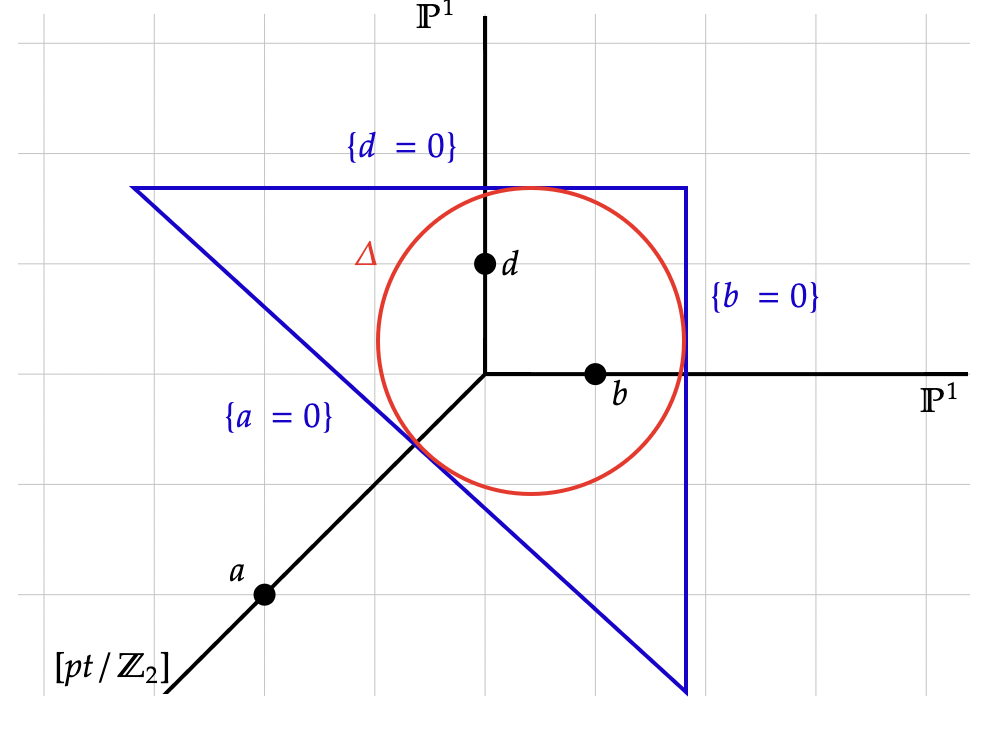
\includegraphics[width=8cm]{rank2exmp/secondarypolytope.png}
    \caption{The blue is a picture of the toric boundary of the secondary toric variety $\Fs$ via orbit-cone correspondence. The lines are the boundary curves $C_W$ of $\Fs$ The discriminant $\Delta$ is red and sits inside $\Fs$. We see that the discriminant locus meets each curve in one point with multiplicity two.}
\end{figure}
\end{comment}
We now explicitly compute the discriminant locus. Recall we scaled out $c$ and $e$. We need to find the $a, b$ and $d$ for which the superpotential
$$
W_{a,b,d}(X,Y,Z) = X(a + bY + Y^{-1} +dZ + Z^{-1})
$$
has critical values. As this problem is simple and our polygon is very symmetric, we can actually do this directly without appealing to more complicated techniques described in \cite{gelfand1994discriminants}. We just need to find the $a,b,d$ for which the partial differential equations have a common zero:
\begin{align}
    \frac{\partial W_{a,b,d}}{\partial X} &= a + bY + Y^{-1} +dZ + Z^{-1}, 
    \label{diff1} \\
    \frac{\partial W_{a,b,d}}{\partial Y} &= b-Y^{-2}, 
    \label{diff2}\\
    \frac{\partial W_{a,b,d}}{\partial Z} &= d - Z^{-2}.
    \label{diff3}
\end{align}
Equation \eqref{diff2} and \eqref{diff3} imply $Y = \pm \frac{1}{\sqrt{b}}$ and $Z = \pm \frac{1}{\sqrt{d}}$, and plugging this into \eqref{diff1} we get
\begin{equation}
    \label{discrimexmp1}
    \Delta = \{d^2 + b^2 + a^4 -2bd - 2a^2b - 2a^2d = 0\}
\end{equation}
\begin{figure}[!h]
    \centering
    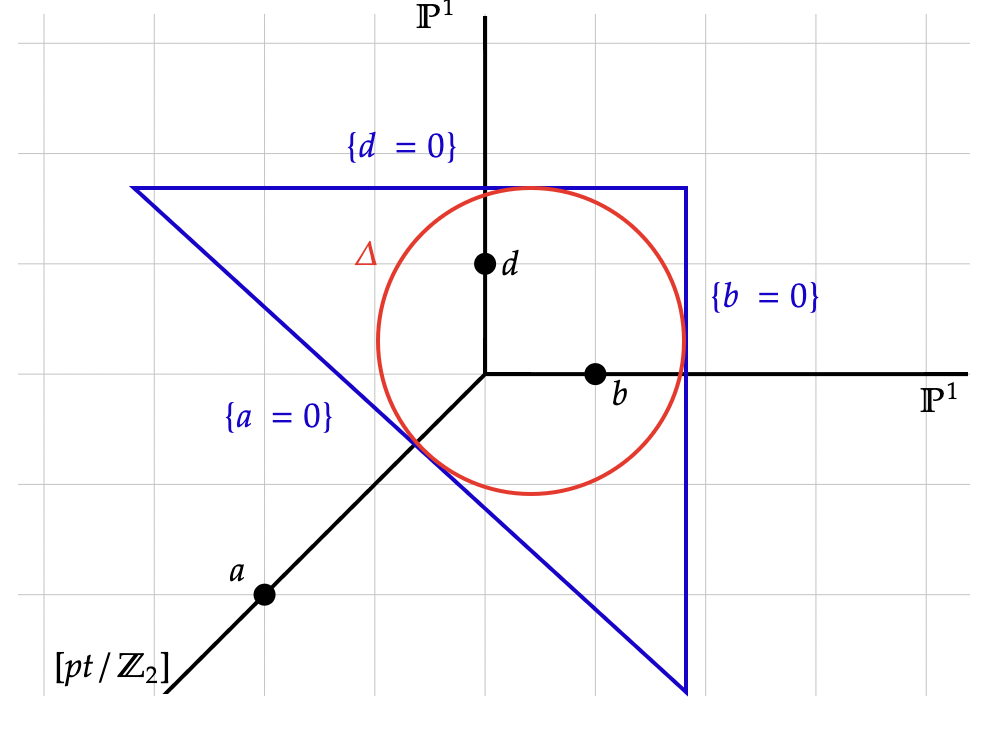
\includegraphics[width=8cm]{rank2exmp/secondarypolytope.png}
    \caption{A picture of $FIPS$ inside the secondary toric variety $\Fs$. The blue is the toric boundary of $\Fs$ via orbit-cone correspondence. The discriminant $\Delta$ is red and sits inside $\Fs$. We see that the discriminant locus meets each curve in one point with multiplicity two by equation \eqref{discrimexmp1}. The variety labels to the walls $W$ are the $Z_W$ from the wall-crossing formula, see Section \ref{wallcrossing}.}
\end{figure}
We will be computing the fundamental group of $FIPS$, where we focus our attention to GIT quotient $X_3$ by picking our base point in $FIPS$ close to the toric fixed point $[0,0,1]\in \Fs$. Following condition (3) in Conjecture \ref{main}, the meridians about $\{a=0 \}$ and $\{b = 0 \}$ should correspond to twisting by line bundles of $X_3$. Recall $X_3 = \left[{\mathcal{O}(-1)^{\oplus 2}}_{\PP^1_{b:c}} / \Z_2 \right]$ with local coordinates on the fibres $d,e$, and we have Picard group
\begin{equation}
\text{Pic} X_3 \cong \Z \oplus \Z_2
\label{picX3}
\end{equation}
where the torsion free part comes from ${\mathcal{O}(-1)^{\oplus 2}}_{\PP^1_{b:c}}$ and $\Z_2$ comes from a choice of representation of the action of $\Z_2$\footnote{The reader may find it helpful to sort of think of coherent sheaves on $X_3$ as finitely generated $\Z \oplus \Z_2$ graded $C[b,c,d,e]$ modules where $d,e$ are in graded piece (-1,-1) and $b,c$ in graded piece (1,0). This is imprecise.}. We represent our line bundles by $\mathcal{O} (n,m)$ where $(n,m) \in \Z \oplus \Z_2$. \\
\newline
In line with this we will scale out $d$ and now think of $FIPS$ as $\left[ (\CC^2 \backslash \{bf(a,b)=0\} ) / \Z_2 \right]$ where $f(a,b)=(a^2 + b )^2 -4a^2b -2(a^2 + b) +1$ and $Z_2$ acts on $a$ by $-1$ and it acts on $b$ trivially. Our choice of base point in the fundamental group will now be a point close to the origin.\\
\newline
What should a meridian around $\{ f(a,b)=0\}$ correspond to? By condition (2) in Conjecture \ref{main}, we want a meridian about discriminant component $\Delta_{\Gamma}$ for $\Gamma \subset P$ a minimal face to correspond to a spherical twisting about a spherical functor $F_{\Gamma}: Z_{\Gamma^c} \to D^b(X_3)$. In this case we only have one non-trivial discriminant component which is $\Gamma = P$. We have $\Gamma^c = \emptyset$ and hence $Z_{\Gamma^c} = pt$. So we want meridians about $\Delta$ to correspond to spherical twists about spherical functors $F: D^b(pt) \to D^b(X_3)$. By our discussion in Section \ref{CY} on spherical functors, this is just a spherical twist about spherical object $F(\Os_{pt})$.\\
\newline 
A priori it seems like we have several spherical functors $F: D^b(pt) \to D^b(X_3)$ coming from the two walls $W_{13}$ and $W_{23}$. For $W_{13}$ the fixed locus under $(0,1)$ is $\{ a=d=e=0 \}$, and we can quotient by the remaining action and find $Z_{13} = \PP^1_{b,c}$. Similarly the fixed locus under $(1,-1)$ is $\{ a=0\}$, and we can quotient by the remaining action and find $Z_{23} = \left[ pt / \Z_2\right]$. Via wall crossing we have two SODs $D^b(Z_{13}) = \langle D^b(pt), D^b(pt) \rangle_{SOD}$ and $D^b(Z_{23}) = \langle D^b(pt), D^b(pt) \rangle_{SOD}$. Looking at the GIT quotient $X_1$ on the other side of $W_{13}$, we see we  remove $\{ d=e=0\}$ instead of $\{ a=0\}$ for $X_3$. In $X_3$, $\{ d=e=0\}$ is just the stacky zero section $\left[\PP^1_{b:c}/ \Z_2 \right]$.
\begin{center}
\begin{tikzcd}
    \left[\PP^1_{b:c}/ \Z_2 \right] \arrow[d,"\pi_{13}"] \arrow[r, "i_{13}"] & X_3 \\
  Z_{13} = \left[ pt / \Z_2\right] &
\end{tikzcd}
\end{center}
Looking at the GIT quotient $X_2$ on the other side of $W_{23}$, we see we  remove $\{ d=e=0\}$ instead of $\{ b=c=0\}$ for $X_3$. Again $\{ d=e=0\}$ is just the stacky zero section $\left[\PP^1_{b:c}/ \Z_2 \right]$.
\begin{center}
\begin{tikzcd}
    \left[\PP^1_{b:c} / \Z_2 \right] \arrow[d,"\pi_{23}"] \arrow[r, "i_{23}"] & X_3 \\
  Z_{23} = \PP^1_{b:c} &
\end{tikzcd}
\end{center}
We have two spherical functors $F_{13} = {i_{13}}_* \pi_{13}^*$ and $F_{23} = {i_{23}}_* \pi_{23}^*$ coming from the walls $W_{13}$ and $W_{23}$, where all these functors are derived. If we restrict these both to the SOD components of $D^b(Z_{13})$ and $D^b(Z_{23})$ we just get spherical object $\Os_{\PP^1}$ twisted by some line bundle, depending on the choice of SOD component. This answers our question:
we will want a a meridian around $\{ f(a,b)=0\}$ to correspond to twisting about $\Os_{\PP^1}$ (or a twist of it). 
\\
\newline
Now that we've explained what meridians should correspond to it's time to compute the fundamental group of $FIPS=\left[ (\CC^2 \backslash \{bf(a,b)=0\} ) / \Z_2 \right]$ with base point near the origin. This is a smooth DM stack and to compute the orbifold  fundamental group, we first remove the $\Z_2$ orbifold curve $\{ a=0\}$ and compute the fundamental group of this non-stacky space. In the group presentation there will be a representative $\gamma$ for the meridian around the stacky locus of the orbifold, and to obtain the orbifold fundamental group we just need to quotient out by $\gamma$ to the power of the order of the finite group acting i.e. $\gamma^2$.\\
\newline
So we compute the fundamental group of $[\CC^2 \backslash \{abf(a,b)=0\}/\Z_2]$. We have a homeomorphism via to $X = \CC^2 \backslash \{abg(a,b)=0\}$ where $g(a,b)=(a + b )^2 -4ab -2(a + b) +1$. We use the Zariski-Van-Kampen method and braid monodromy techniques for computing the fundamental group of curve complements. The first thing we need to do this is to choose a projection to $\CC^1$ which is almost everywhere a locally trivial fibration. This is explained well in \cite{cogolludo}. In Figure \ref{FIPS1} we see the real picture of $X$, where the parabola intersects both axes at tacnodes $(0,1)$ and $(1,0)$.
\begin{figure}[!h]
    \centering
    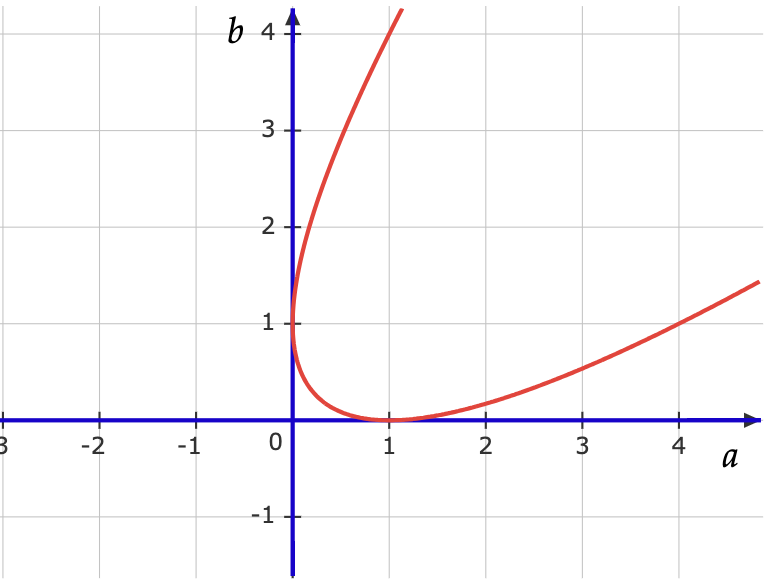
\includegraphics[width=8cm]{rank2exmp/FIPS1.png}
    \caption{Real picture of $X$.}
    \label{FIPS1}
\end{figure}
\\
\newline
We have a choice of which projection to use, but the best projection is one where we can maximally exploit what we see in the real picture. For example, ideally we want a projection where we can see all non-generic fibres in the real picture. We also want a projection where all the points missing from generic real fibres are in the real picture. This is not necessarily always possible, but in this example it is by projecting onto $\{ a=-b \}$. We therefore consider the projection $X \xrightarrow[]{\pi} \CC^1$, defined as $(a,b) \mapsto a-b$, where the fibres are lines in $\CC^2_{a,b}$ of gradient 1.
\begin{figure}[!h]
    \centering
    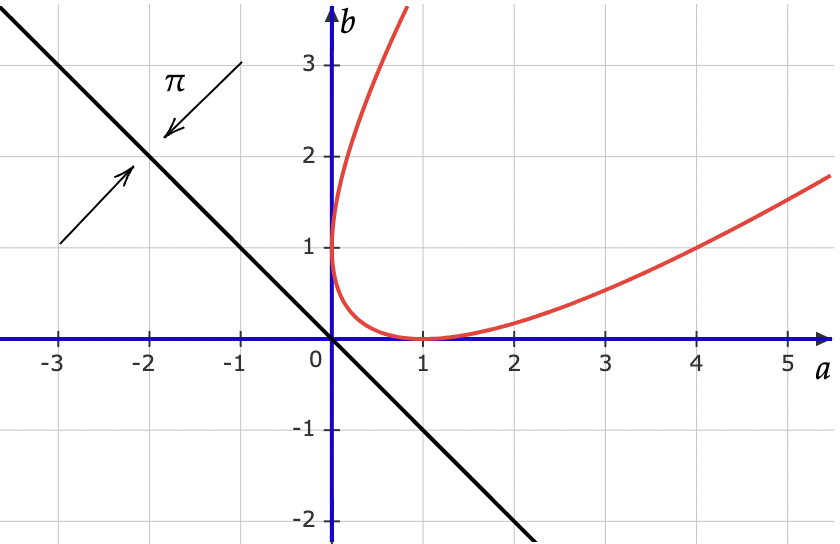
\includegraphics[width=8cm]{rank2exmp/projection1.png}
    \caption{The projection $\pi$ of X in the real picture.}
    \label{projection1}
\end{figure}
We can see that $\pi$ is a locally trivial fibration outside of the three special fibers:
\begin{itemize}
    \item $L_1 = \pi^{-1}(z_1)$, the fiber containing the tacnode at (0, 1), \\
    \item $L_2 = \pi^{-1}(0)$, the fiber containing the node at (0, 0), \\
    \item $L_3= \pi^{-1}(1)$, the fiber containing the tacnode at (1, 0).
\end{itemize}
Our first step will be to compute the fundamental group of $X$ without the special fibres. We will do this by the following theorem.
\begin{thm}\cite[Theorem 2.1]{cogolludo}
\label{locallytriv}
Suppose you have a locally trivial fibration $\pi : M \to N$ with section $s : N\to M$ and take $p \in N $. Let $F = \pi^{-1}(p)$ be the fibre over $p$, and $x\in F\subset X$. Then $\pi_1(M,x) = \pi_1(F,x) \rtimes \pi_1(N,p)$, where the action of $\pi_1(N,p)$ on $\pi_1(F,x)$ is given by monodromy. 
\end{thm}
\begin{figure}[!h]
    \centering
    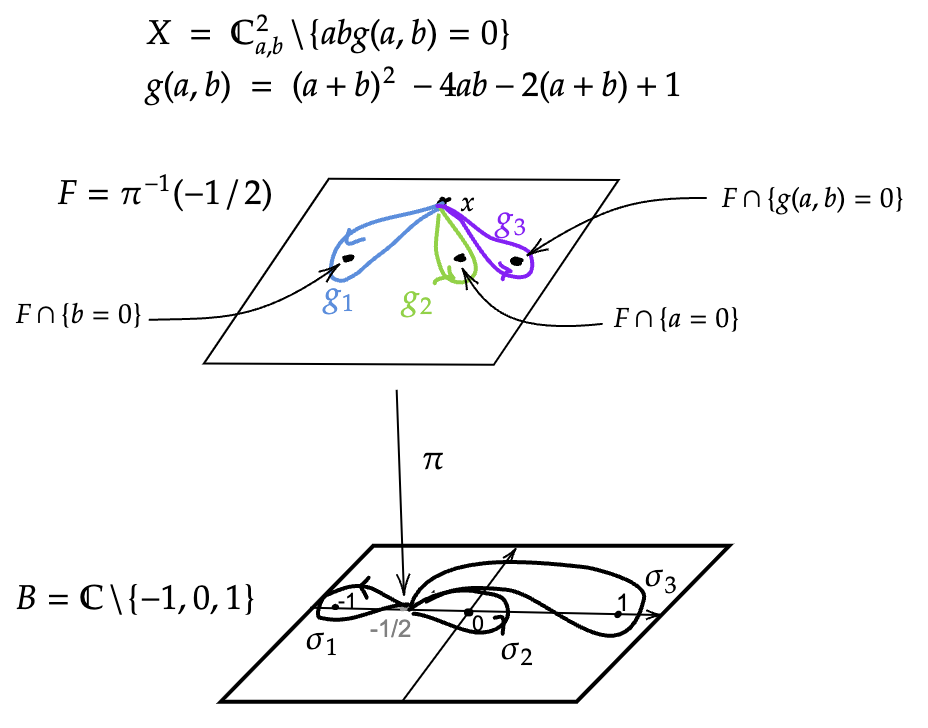
\includegraphics[width=12cm]{rank2exmp/zariski1.png}
    \caption{Loops in $Y$.}
    \label{zariski1}
\end{figure}
We restrict our $\pi$ to the aforementioned locally trivial fibration. Let $Y= X \backslash L_1 \cup L_2 \cup L_3$. $\pi : Y  \to \CC^1\backslash \{-1,0,1 \}$. It is easy to see that this now a locally trivial fibration (see Figure \ref{zariski1}). We denote the base $\CC^1\backslash \{-1,0,1 \}$ by $B$. Each fibre of $\pi$ is now homeomorphic to $\CC^1 \backslash \{3 pts\}$. We consider loops $\sigma_1,\sigma_2, \sigma_3 \in \pi_1(B,-1/2)$ that freely generate the fundamental group on the the base $B$ with base point $-1/2 \in B$. Let $F=\pi^{-1}(-1/2)\cong \CC^1\backslash \{ 3 pts\}$ be the fibre of $\pi$ above this basepoint. We choose a basepoint $x \in F \subset X$ in the fibre to be quite far from the three missing points\footnote{More specifically we need to pick $x \in X$ far enough so that if $A\subset F$ is a bounded closed subset containing the paths traced out by the missing points in the fibres as we move along the loops $\sigma_i$ on the base, then $x \in B\backslash A$. We want this so that later we can easily argue that gluing the special fibres back in and computing $\pi_1(X)$ just amounts to trivialising the $\sigma_i$.}. The loops $g_1,g_2,g_3 \in \pi_1(F,x)$ around the missing points in the fibre coming from $\{b=0 \}$, $\{ a=0\}$, and $\{g(a,b)=0\}$ respectively freely generate the fundamental group of the fibre with base point $x \in X$. The missing points are precisely the points of intersection of the curves in Figure \ref{FIPS1} with the line $b=a-1/2$. As we move along the loops $\sigma_i$ on the base we have a monodromy action on $g_1,g_2,g_3$. This monodromy action arises from the continuous trajectory of the missing points in the fibres as we move along loops on the base through the homotopy lifting property of locally trivial fibrations. We shall denote the loops after after monodromy ${g_j}^{\sigma_i}$. By Theorem \ref{locallytriv} we have group presentation for the fundamental group of $Y$:
\begin{align*}
    \pi_1(Y,x) &\cong \pi_1(F,x) \rtimes \pi_1(B,-1/2)  \\
    &=\langle \, g_1,g_2,g_3,\sigma_1,\sigma_2,\sigma_3 \, | \,\forall i,j \in \{1,2,3 \}, \: \: \: {g_j}^{\sigma_i}={\sigma_i}^{-1} g_j \sigma_i \, \rangle
\end{align*}
So we now need to understand ${g_j}^{\sigma_i}$. As we move around $\sigma_i$ the three points missing in the fibre move. Let us parametrise $\sigma_i$ by $t \in [0,1 ]$. Braid monodromy techniques become useful because in $\pi^{-1}(\sigma_i([0,1]))$, the missing points actually form 3 strands of a braid. The local monodromy can be worked out from the braid. \\
\newline
We work this out explicitly for the loop $\sigma_1\in \pi_1(B,-1/2)$. Locally near $-1 \in B$, our fibration is equivalent to the locally trivial fibration 
$$\tau : \CC^2_{x,y}\backslash \{ y=-2, y=0, y=x^2\} \to \CC_x^*.$$
Here we can take $\sigma_1(t) = e^{2\pi it} \in \CC_x^*$ and $\{ y=-2\}$, $\{y=0\}$ and $\{y =x^2\}$ correspond to the curves $\{b=0\}$, $\{a=0\}$ and $\{ g(a,b)=0\}$. 
\begin{figure}[!h]
    \centering
    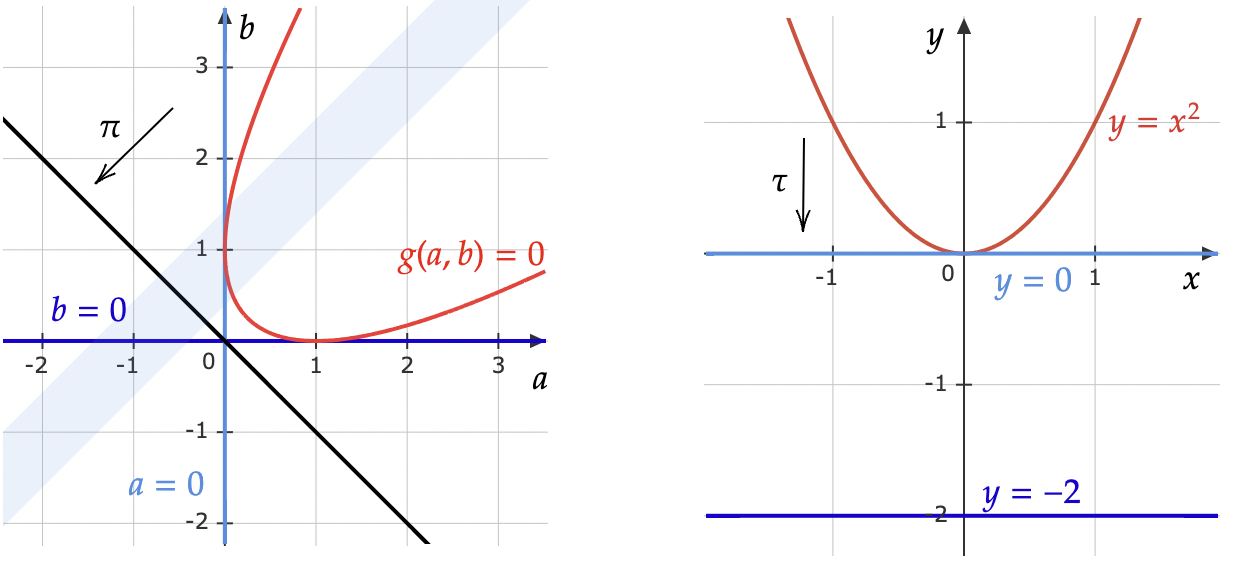
\includegraphics[width=12cm]{rank2exmp/exmp1tau.png}
    \caption{The locally trivial fibration $\pi: Y \to B$ locally around $-1 \in B$.}
\end{figure}
\\
We can see the associated braid on three strands in Figure \ref{sigma1}.
\begin{figure}[!h]
    \centering
    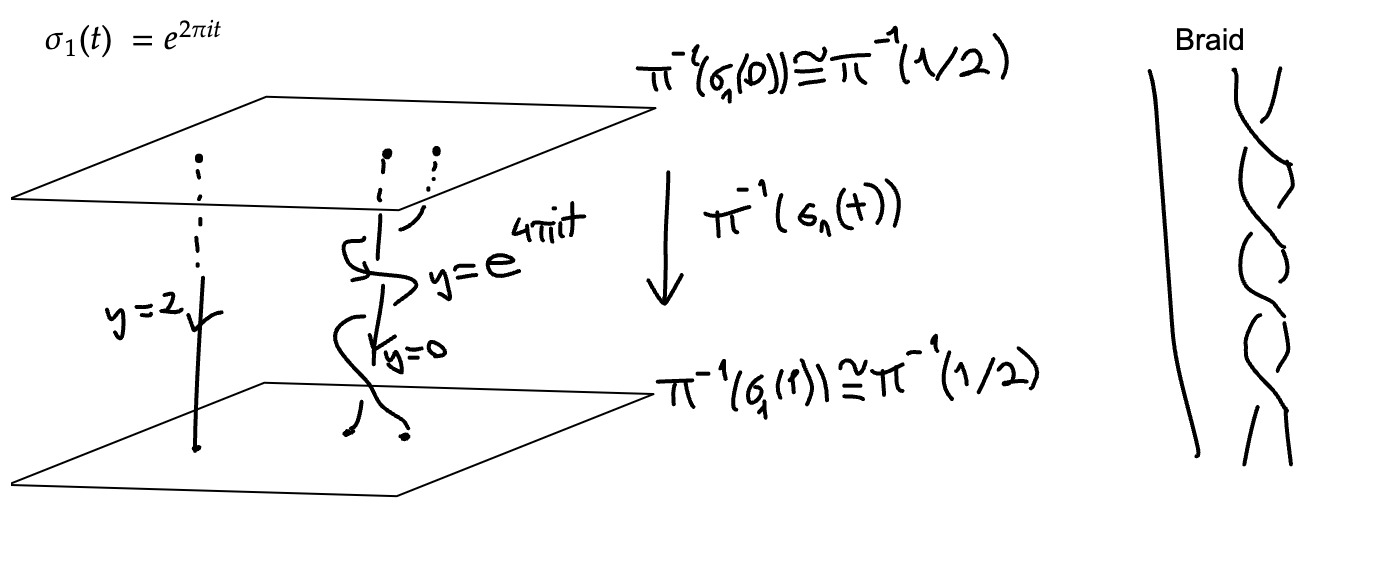
\includegraphics[width=12cm]{rank2exmp/sigma1.png}
    \caption{The braid associated to $\sigma_1$.}
    \label{sigma1}
\end{figure}
The loops $g_1,g_2,g_3$ in the fibre $F$ move along the strands and where they end up is precisely the braid monodromy action of $\sigma_1$. We draw the movement of the loops along the braids in Figure \ref{braidaction1}.
\begin{figure}[!h]
    \centering
    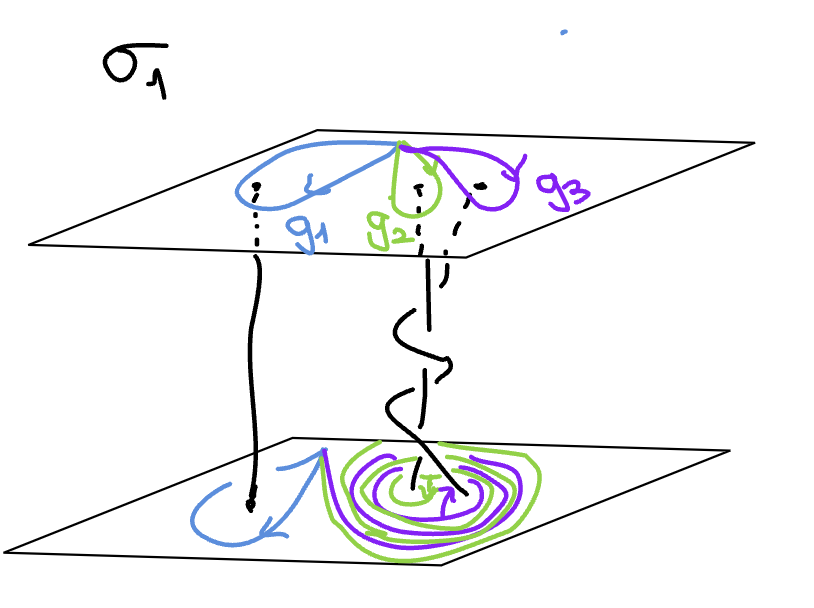
\includegraphics[width=8cm]{rank2exmp/braidaction1.png}
    \caption{The braid monodromy action of $\sigma_1$ on $g_1,g_2,g_3$.}
    \label{braidaction1}
\end{figure}
In the same way as we see exhibited in Figure \ref{braidaction1}, any braid on 3 strands acts on $\pi_1(F,x)$. Also, any loop on the base corresponds to a braid up to homotopy. We recall that $B_3$ is generated by braids $b_1$ and $b_2$ and has presentation $B_3 = \langle b_1,b_2 | b_1 b_2 b_1 = b_2 b_1 b_2\rangle$.
\begin{figure}[!h]
    \centering
    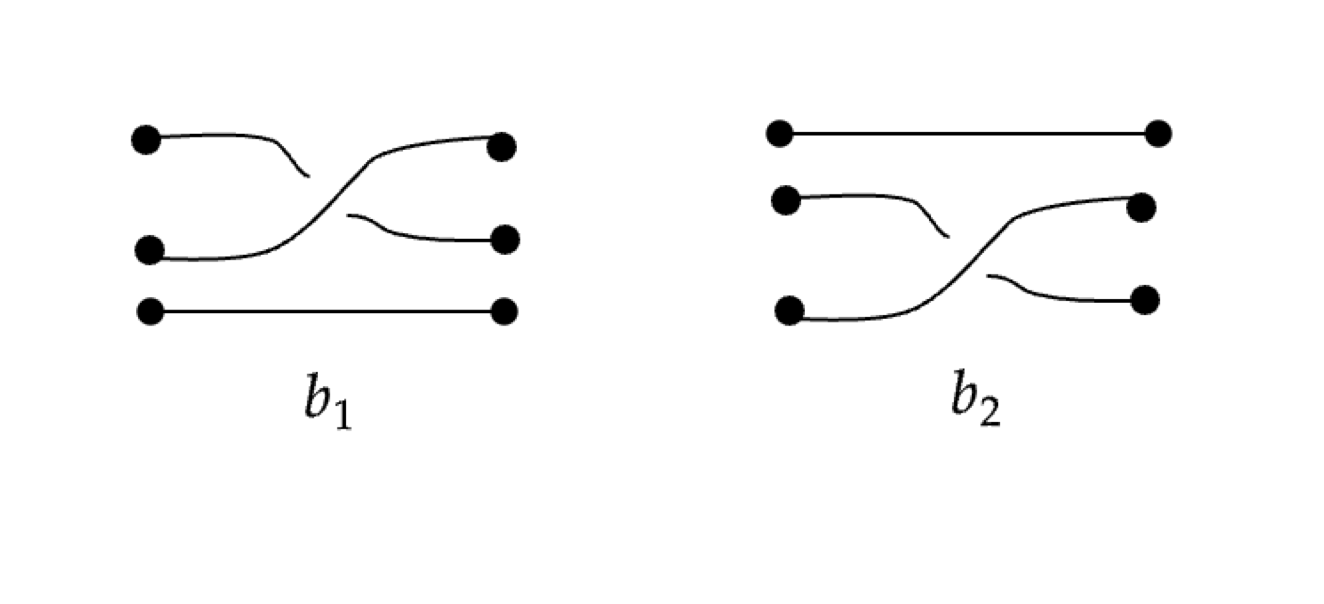
\includegraphics[width=8cm]{rank2exmp/B3.png}
    \caption{The standard generators of the braid group on three stands $B_3$.}
    \label{braidgenerators}
\end{figure}\\
\newline
In Figure \ref{sigma1} we see that the braid for $\sigma_1$ is $(b_1)^4$. With reference to Figure \ref{braidgenaction} the braid $b_1$ acts on $g_1$, $g_2$, and $g_3$ by
\begin{align*}
    g_1 &\mapsto g_1 \\
    g_2 &\mapsto g_2 g_3 {g_2}^{-1} \\
    g_3 &\mapsto g_2 
\end{align*}
and the braid $b_2$ acts on $g_1$, $g_2$, and $g_3$ by
\begin{align*}
    g_1 &\mapsto g_1 g_2 {g_1}^{-1} \\
    g_2 &\mapsto g_1 \\
    g_3 &\mapsto g_3
\end{align*}
\begin{figure}[!h]
    \centering
    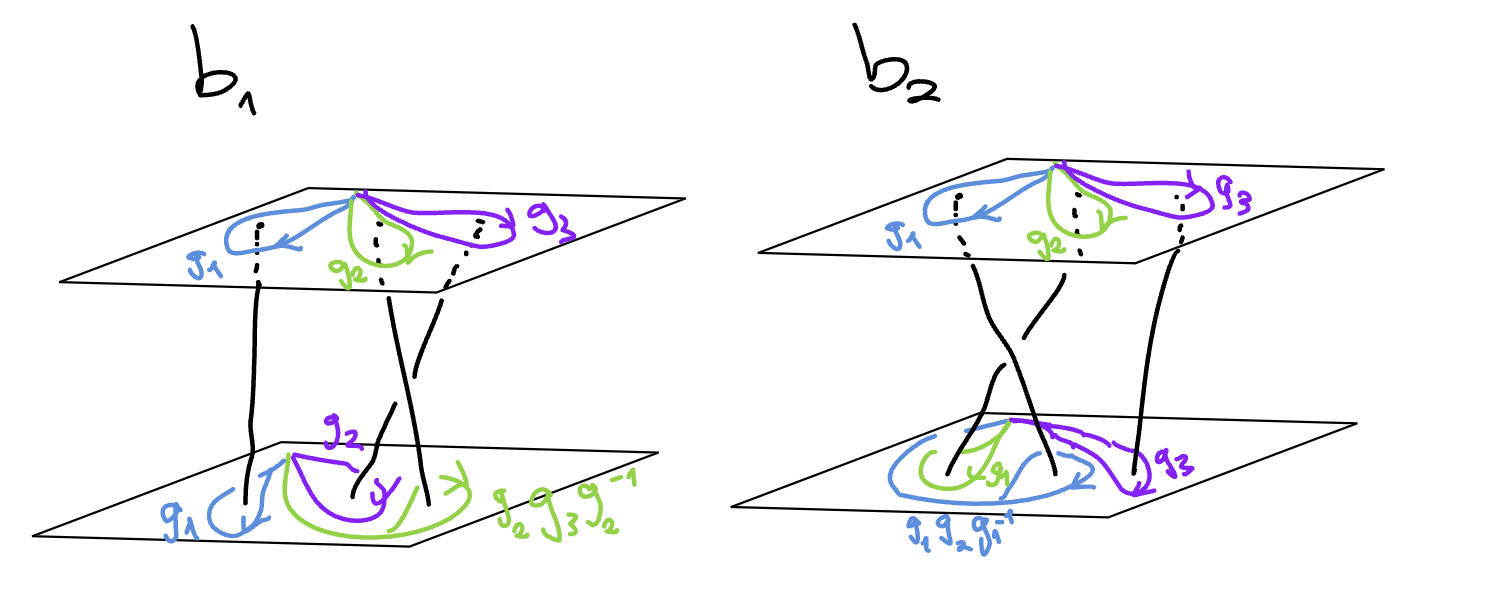
\includegraphics[width=14cm]{rank2exmp/braidgenerators.png}
    \caption{The actions of $b_1$ (left) and $b_2$ (right) on loops $g_1,g_2,g_3$}
    \label{braidgenaction}
\end{figure}
A quick computation shows that the local action of $\sigma_1 = (b_1)^4$ is 
\begin{align*}
    g_1 &\mapsto g_1, \\
    g_2 &\mapsto (g_2 g_3 g_2 g_3) g_2 (g_2 g_3 g_2 g_3)^{-1}, \\
    g_3 &\mapsto (g_2 g_3 g_2) g_3 (g_2 g_3 g_2)^{-1}, 
\end{align*}
We can compute the local monodromy of $\sigma_2$ and $\sigma_3$ in the same way, by looking at our locally trivial fibration locally. A crucial point is that looking locally only gives us the local monodromy, but not the global one\footnote{Computing the global monodromy is where the real issues with computing the fundamental group of curve complements comes from.}. Given our choice of base point, our computation of the local monodromy $\sigma_1$ and $\sigma_2$ will be the global one. This is not true for $\sigma_3$. \\
\newline
Repeating the process above we get that the local braid $\sigma_2$ is ${b_2}^2$. For $\sigma_2$ the local braid is all we need to compute the global monodromy action due to our choice of base point on $B$. For $\sigma_3$ the local monodromy braid is also ${b_1}^4$ (just like for $\sigma_1$, which makes sense given the symmetry of $X$ and our fibration). But the local braid is not enough to give us the global monodromy action because to get from our base point $-1/2 \in B$ to a base point in the the local locally trivial fibration picture around $1 \in B$ we need to transverse the loop $\sigma_2$ half way, and then we need to bring it back through that segment of $\sigma_2$ again. In other words, since $\sigma_2 = {b_2}^2$, our global braid is going to be $\sigma_3 = b_2 {b_1}^4 {b_2}^{-1}$. We can now finally write down what ${g_i}^{\sigma_j}$ are:
\begin{align*}
    {g_1}^{\sigma_1} &= g_1, \\
    {g_2}^{\sigma_1} &= (g_2 g_3 g_2 g_3) g_2 (g_2 g_3 g_2 g_3)^{-1} \\
    {g_3}^{\sigma_1} &= (g_2 g_3 g_2) g_3 (g_2 g_3 g_2)^{-1}, \\ 
    {g_1}^{\sigma_2} &= (g_1g_2) g_1 (g_1 g_2)^{-1},\\
    {g_2}^{\sigma_2} &= g_1 g_2 {g_1}^{-1},\\
    {g_3}^{\sigma_2} &= g_3, \\
    {g_1}^{\sigma_3} &= (g_1 g_3 g_1 g_3) g_1 (g_1 g_3 g_1 g_3)^{-1}, \\
    {g_2}^{\sigma_3} &= (g_1 g_3 g_1 g_3)(g_3 g_1 g_3 g_1)^{-1} g_2 (g_3 g_1 g_3 g_1)(g_1 g_3 g_1 g_3)^{-1}, \\
    {g_3}^{\sigma_3} &= (g_1 g_3 g_1)g_3 (g_1 g_3 g_1)^{-1}, 
\end{align*}
We are finally now ready to write a presentation for the fundamental group of $\pi_1(X,x)$. By the Zariski-Van Kampen Theorem \cite[Theorem 2.6 ]{cogolludo}, gluing the special fibres $L_i$ back into $Y$ trivialises the loops on the base $\sigma_i$. So we have 
$$
\pi_1(X,x) = \langle g_1, g_2, g_3 | {g_i}^{\sigma_j}=g_i, i,j \in \{1,2,3\} \rangle.
$$
Simplifying the relations we get a simple presentation of $\pi_1(X,x)$,
$$
\pi_1(X,x) = \langle g_1, g_2, g_3 | g_1g_2=g_2 g_1, (g_1 g_3)^2 = (g_3 g_1)^2 , (g_2g_3)^2= (g_3g_2)^2\rangle.
$$
This is also known as the even Artin group $\A (2,4,4)$. To get the orbifold fundamental group of $\pi_1(FIPS)$ recall we have to quotient by the square of the meridian about $\{ a=0\}$, which is represented by $g_2$. So 
\begin{align}
\pi_1(FIPS) = \langle g_1, g_2, g_3 |(g_3g_2)^2 = (g_2g_3)^2, [g_1,g_2]=1, (g_1 g_3)^2 = (g_3 g_1)^2 , {g_2}^2 =1\rangle.
\label{fipspresentation}
\end{align}
We go back to our story where $\pi_1(FIPS)$ acts via autoequivalence on the bounded derived category of our phase $X_3 = \left[{\mathcal{O}(-1)^{\oplus 2}}_{\PP^1_{b:c}} / \Z_2 \right]$ with local coordinates on the fibres $d,e$. Recall that the meridians $ g_1$ and $g_2$ about $\{b=0 \}$ and $\{a=0 \}$ should correspond to line bundle twists, and the meridian $ g_3 $ about the discriminant locus $\Delta$ corresponds to doing a spherical twist about the spherical object $S=\Os_{\PP^1}$. We recall from Equation \eqref{picX3} the structure of $\text{Pic}X_3$, and set
\begin{align*}
    g_1 &= \otimes \Os(1,0) : D^b(X_3) \to D^b(X_3),\\
    g_2 &= \otimes \Os(0,1) : D^b(X_3) \to D^b(X_3)\\
    g_3 &= T_{S}: D^b(X_3) \to D^b(X_3),
\end{align*}
where we recall the definition of a spherical twist about a spherical object $S \in D^b(X_3)$:
\begin{equation*}
     T_{S}\Es =C\left(\text{Hom}(S,\Es )\otimes S \to \Es  \right).
\end{equation*}
To check that the fundamental group does act in this way, we need to verify that the functors assigned satisfy the group relations. We will exploit the following easy lemma.
\begin{lemma}
    \label{twistrels}
    Let $F : \mathcal{A} \to \mathcal{B}$ be a spherical functor between triangulated categories and let $\Phi : \mathcal{B} \to \mathcal{B}$ be an autoequivalence. Then
    $$
    \Phi \circ T_F \circ  \Phi^{-1} = T_{\Phi \circ F}.
    $$
\end{lemma}
\begin{proof}
    The proof is obvious.
\end{proof}
The second relation and the fourth relation in the presentation for $\pi_1(FIPS)$ (Equation \eqref{fipspresentation}) are obvious since tensoring by line bundles is commutative and we know that $\Os(0,1)$ is 2-torsion. The first and third relations can be rewritten:
\begin{align*}
    g_3 g_2 g_3 {g_2}^{-1} {g_3}^{-1} &= {g_2}^{-1}g_3 g_2,\\
    g_3 g_1 g_3 {g_1}^{-1} {g_3}^{-1} &= {g_1}^{-1}g_3 g_1 .
\end{align*}
Substituting in our functors and using Lemma \ref{twistrels} the relations read:
\begin{align*}
    T_{T_{S} {\Os_{\PP^1}(0,1)}} &= T_{\Os_{\PP^1}(0,1)},\\
    T_{T_{S} \Os_{\PP^1}(1,0)} &= T_{\Os_{\PP^1}(-1,0)}.
\end{align*}
where we used that $\Os(0,1)^{-1} = \Os(0,1)$. Therefore if we show
\begin{align}
    T_{S} \Os_{\PP^1}(0,1)&= \Os_{\PP^1}(0,1), 
    \label{rel1}\\
    \label{rel2} T_{S} \Os_{\PP^1}(1,0) &= \Os_{\PP^1}(-1,0),
\end{align}
then we're done. Let's start by computing $T_{\Os_{\PP^1}}\Os_{\PP^1}(0,1)$. We note that\footnote{In the second equality we use that the local-to-global spectral sequence terminates on the second page, which is easy to argue.}
\begin{align*}
    \text{RHom}(\Os_{\PP^1}(k_1, k_2),\Os_{\PP^1}(m_1,m_2)) &= \text{RHom}(\Os_{\PP^1},\Os_{\PP^1}(m_1 - k_1, m_2 - k_2)), \\
    &=R\Gamma \left(\text{R}\mathcal{H}om(\Os_{\PP^1},\Os_{\PP^1})(m_1 - k_1, m_2 - k_2) \right).
\end{align*}
So we start by computing $\text{R}\mathcal{H}om(\Os_{\PP^1},\Os_{\PP^1})$, then we twist it accordingly and take deried global sections (sheaf cohomology). To compute the derived functor we start by Koszul resolving $\Os_{\PP^1}$:
\begin{equation*}
0 \xrightarrow[]{} \Os(2,0) \xrightarrow[]{(-e,d)} \Os(1,1)^2\xrightarrow[]{(d,e)^T} \Os \xrightarrow[]{} \Os_{\PP^1} \xrightarrow[] {}0
\end{equation*}
Ignore $\Os_{\PP^1}$ in the resolution and taking $\mathcal{H}om(, \Os_{\PP^1})$ we get
\begin{equation}
\label{koszul}
\text{R}\mathcal{H}om(\Os_{\PP^1},\Os_{\PP^1}) = 0 \xleftarrow[]{} \Os_{\PP^1}(-2,0) \xleftarrow[]{0} \Os_{\PP^1}(-1,1)^2\xleftarrow[]{0} \Os_{\PP^1} \xleftarrow[]{} 0
\end{equation}
We twist by $\Os(0,1)$:
$$
0 \xleftarrow[]{} \Os_{\PP^1}(-2,1) \xleftarrow[]{0} \Os_{\PP^1}(-1,0)^2\xleftarrow[]{0} \Os_{\PP^1}(0,1) \xleftarrow[]{}0
$$
We take derived global sections and get 0 in all degrees. For $\Os_{\PP^1}(-2,1)$ we can see this because there is only one extension (of degree 1) of $\Os_{\PP^1}(-2)$ in $\PP^1$, and in $[ \PP^1 / \Z_2 ]$ it is not $\Z_2$ invariant:
$$
0 \xrightarrow[]{} \Os_{\PP^1}(0,1) \xrightarrow[]{\begin{pmatrix}
    c & -b
\end{pmatrix}} \Os_{\PP^1}(-1,1)^2\xrightarrow[]{\begin{pmatrix}
    b \\
    c
\end{pmatrix}} \Os_{\PP^1}(-2,1) \xrightarrow[]{}0
$$
For $\Os_{\PP^1}(-1,0)$ we know $\Os_{\PP^1}(-1)$ in $\PP^1$ has no sheaf cohomology. For $\Os_{\PP^1}(0,1)$ the derived global sections come from genuine sections of $\Os_{\PP^1}$ in $\PP^1$ i.e. degree 0 polynomials in $b,c$ variables (constants), but these are $\Z_2$ invariant.
So $\text{RHom}\left(\Os_{\PP^1},\Os_{\PP^1}(0,1)\right) = 0$ and we have
$$
T_{\Os_{\PP^1}}\Os_{\PP^1}(0,1) = C(0 \to \Os_{\PP^1}(0,1)) =\Os_{\PP^1}(0,1),
$$
which is precisely the relation \eqref{rel1}. To check the relation \eqref{rel2} we twist \eqref{koszul} by $\Os(1,0)$:
\begin{equation*}
0 \xleftarrow[]{} \Os_{\PP^1}(-1,0) \xleftarrow[]{0} \Os_{\PP^1}(0,1)^2\xleftarrow[]{0} \Os_{\PP^1}(1,0) \xleftarrow[]{0} 0
\end{equation*}
Taking global sections we get $\CC^2_{b,c}$ in degree 0. So
$$
T_{\Os_{\PP^1}}\Os_{\PP^1}(1,0) = C({\Os_{\PP^1}}^2 \to \Os_{\PP^1}(1,0)) =\Os_{\PP^1}(-1,0),
$$
using the Euler sequence. This is relation \eqref{rel2}.
\section{Toric Calabi-Yau threefolds of Picard rank 2}
\label{future}
In the rank 2 example we presented in Section \ref{rank2example}, the GIT quotient $X_1$ is a toric Calabi-Yau threefold of Picard rank 2. Given any toric Calabi-Yau threefold $X$ of Picard rank 2, we can consider the brane monodromy conjecture by constructing a toric Calabi-Yau GIT problem $(\CC^*)^2$ acting on $\CC^5$ for which $X$ is a GIT quotient. Note that we know the rank of the GIT problem 2 because of the rank of the Picard group, and we know the dimension of the problem is 5 because the quotient $X$ is three-dimensional. Suppose the problem is given by exact sequence
$$
\Z^3 \xrightarrow{A} \Z^5 \xrightarrow{Q} \Z^2
$$
where $Q$ is the weight matrix. Recall from Section \ref{fips} the definition of the primary polygon $P \in \Z^3 \otimes_{\Z} \R$, which is the convex hull of the rays $a_i = A^T(e_i) \in \Z^{3}$. Different triangulations of the primary polygon correspond precisely to the different GIT quotients, in that the cone on the triangulated polygon gives you the toric fan of your quotient. Since we could have chosen a different set of generators for $\text{ker}Q \cong \Z^3$, we have an action by $GL_3(\Z)$ on this polygon. Because of our Calabi-Yau assumption (the weights sum up to 0), we can choose generators so that the column of $A$ is a list of 1s, and we see $P$ living in the rank 2 lattice in $\Z^3$ where the first integer coordinate is 1. \\
\newline
Even if we impose the first column of $A$ to be 1, we still have a residual action on $P$. The matrices in $GL_3(\Z)$ that keep the polyton's first coordinate 1 are given in block form:

\[
\begin{pNiceArray}{c|c}
  1 & \begin{array}{c c } 
    t_1 & t_2
 \end{array} \\
  \hline
  \begin{array}{c c } 
    0 \\
    0
 \end{array} & M
\end{pNiceArray}
\]
where $t_1,t_2 \in \Z$ and $M \in GL_{2} (\Z)$. This means we consider $P\subset \Z^2$ up to $GL_{2} (\Z)$ and translations. \\
\newline
Because we know $A^T$ is surjective, we know that the primary polytope has exactly 5 integer points in it. This means that toric Calabi-Yau threefold of Picard rank 2 come from convex polygons in $\Z^2$ with exactly 5 integer points, up to the $GL_{2} \Z \times \Z^2$ action. We have proved that there are only six such classes of  polygons, see Figure \ref{CY3rank2}.
\begin{figure}[!h]
    \centering
    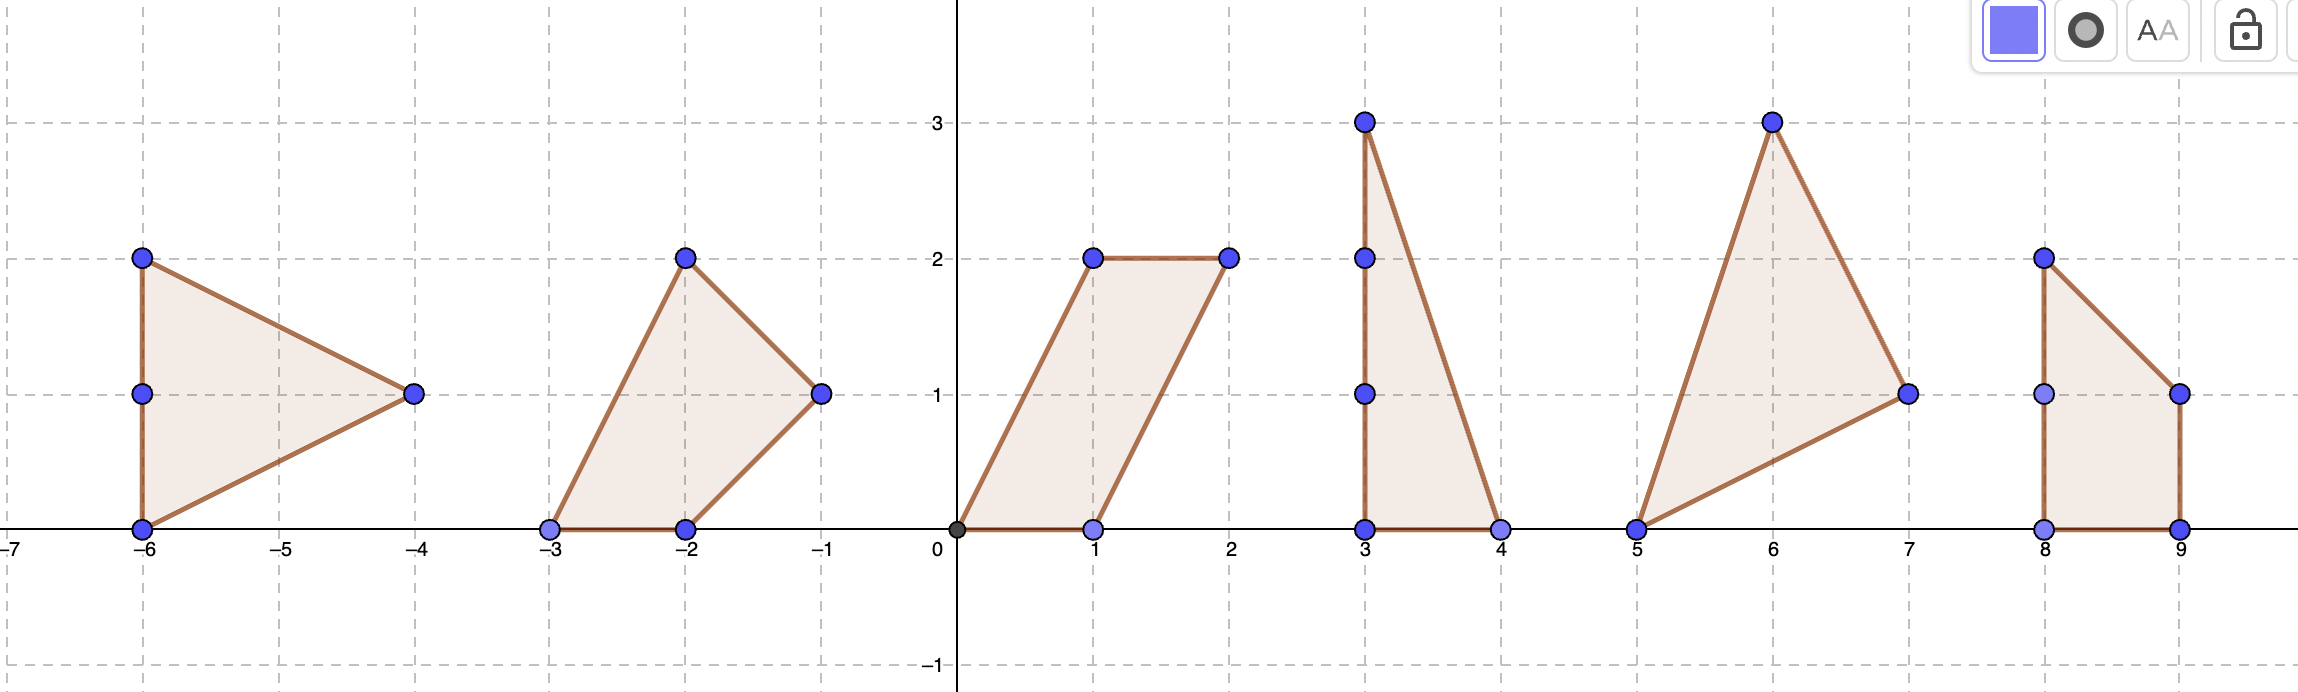
\includegraphics[width=12cm]{3foldsofpicardrank2.png}
    \caption{The toric Calabi-Yau threefolds of Picard rank 2.}
    \label{CY3rank2}
\end{figure}
The third polygon in Figure \ref{CY3rank2} actually corresponds to our example in Section \ref{rank2example}. The fourth and sixth polygon examples have been worked out in \cite{edwill} as part of another class of examples. I have also done the computation for the first polygon, which we note would give an example where we have more than one discriminant component as there are two minimal faces. To complete this project I need to work out the conjecture for the second and fifth polygons. Though these examples only have one discriminant component, they should be harder because we can't compute the discriminant locus directly. We will need to use Cayley method, presented in \cite[Chapter 2]{gelfand1994discriminants}. Once we have the curves the fundamental group computation should be harder than those in the examples far, since our curves have been exceptionally nice (the components smooth, with good real pictures). It's my hope that these examples will exhibit some new and interesting behaviour. \\
\newline
I also have shown that there are only finitely many toric Calabi-Yau threefolds for any given rank, so in principle we could carry out this program for Picard rank 3. \\
\newline
We also note that this problem has been solved for a special class of toric CY GIT problems called \textit{quasi-symmetric} \cite{quasi-sym}. I am thinking about whether this result can be used to generalise to other examples by embedding the data of our GIT problem into a quasi-symmetric one. I am also thinking about whether we can say something about some non-abelian GIT quotients. 
\bibliographystyle{abbrv}
\bibliography{mybib.bib}


\end{document}